% \documentclass[a4paper,10pt]{article} % or whatever
% \documentclass[letterpaper,10pt]{article} % or whatever
\documentclass{article}

% if you need to pass options to natbib, use, e.g.:
     \PassOptionsToPackage{numbers, compress}{natbib}

\usepackage[preprint]{neurips_2021}

\newcommand{\ignore}[1]{}
% to avoid loading the natbib package, add option nonatbib:
\usepackage{dsfont}

% Note: this has been tested using MiKTeX 2.9. If you are getting errors, update your packages.

%%% Packages %%%
%\usepackage{setspace} % Double spaces document. Footnotes,
                      % figures, and tables will still be single spaced, however.
%\doublespacing
%\singlespacing
%\onehalfspacing
% \setstretch{1.5} % set double spacing to 1.5 or anything else.

\usepackage[T1]{fontenc}
\usepackage{amsmath,amssymb,amsfonts,mathrsfs,bm}% Typical maths resource packages
\usepackage{mathtools}
%\let\proof\relax
%\let\endproof\relax
\usepackage{amsthm}
\usepackage{nicefrac}
%\usepackage{cite}
%\let\labelindent\relax
\usepackage[shortlabels]{enumitem}
\usepackage{graphicx}
\usepackage{epstopdf}
\usepackage{url}
\usepackage{colortbl}
\usepackage{booktabs}
\usepackage{multirow}
\usepackage[table,dvipsnames]{xcolor}
\usepackage[normalem]{ulem}
\usepackage{xparse}

%\usepackage{pstricks}
%\usepackage{psfrag}
%\usepackage{syntonly}
%\syntaxonly
%\usepackage[style=base]{caption}
%\captionsetup{
    %format = plain,
    %font = footnotesize,
    %labelfont = sc
%}


\usepackage{array}
\newcolumntype{L}[1]{>{\raggedright\let\newline\\\arraybackslash\hspace{0pt}}m{#1}}
\newcolumntype{C}[1]{>{\centering\let\newline\\\arraybackslash\hspace{0pt}}m{#1}}
\newcolumntype{R}[1]{>{\raggedleft\let\newline\\\arraybackslash\hspace{0pt}}m{#1}}

\makeatletter
\let\MYcaption\@makecaption
\makeatother
\usepackage[font=footnotesize]{subcaption}
\makeatletter
\let\@makecaption\MYcaption
\makeatother


% achieves the functionality of \tag for subequations environment
\makeatletter
\newenvironment{varsubequations}[1]
 {%
  \addtocounter{equation}{-1}%
  \begin{subequations}
  \renewcommand{\theparentequation}{#1}%
  \def\@currentlabel{#1}%
 }
 {%
  \end{subequations}\ignorespacesafterend
 }
\makeatother


\usepackage{glossaries}

\makeatletter
% copy old \gls and \glspl
\let\oldgls\gls
\let\oldglspl\glspl

% define a non space skipping version of \@ifnextchar
\newcommand\fussy@ifnextchar[3]{%
  \let\reserved@d=#1%
  \def\reserved@a{#2}%
  \def\reserved@b{#3}%
  \futurelet\@let@token\fussy@ifnch}
\def\fussy@ifnch{%
  \ifx\@let@token\reserved@d
    \let\reserved@c\reserved@a 
  \else
    \let\reserved@c\reserved@b
  \fi
 \reserved@c}

\renewcommand{\gls}[1]{%
  \oldgls{#1}\fussy@ifnextchar.{\@checkperiod}{\@}}
\renewcommand{\glspl}[1]{%
  \oldglspl{#1}\fussy@ifnextchar.{\@checkperiod}{\@}}

\newcommand{\@checkperiod}[1]{%
  \ifnum\sfcode`\.=\spacefactor\else#1\fi
}
\makeatother

%%%%%%%%%%%%% new add %%%%%%%%%%%%% 
\newcommand{\tb}[1]{\textbf{#1}}


\newacronym{wrt}{w.r.t.}{with respect to}
\newacronym{RHS}{R.H.S.}{right-hand side}
\newacronym{LHS}{L.H.S.}{left-hand side}
\newacronym{iid}{i.i.d.}{independent and identically distributed}
%\newacronym{MIMO}{MIMO}{mulitple-input multiple-output}
%\newacronym{AOA}{AOA}{angle-of-arrival}
%\newacronym{AOD}{AOD}{angle-of-departure}
%\newacronym{LOS}{LOS}{line-of-sight}
%\newacronym{NLOS}{NLOS}{non-line-of-sight}
%\newacronym{TOA}{TOA}{time-of-arrival}
%\newacronym{TDOA}{TDOA}{time-difference-of-arrival}
%\newacronym{RSS}{RSS}{received signal strength}
%\newacronym{GNSS}{GNSS}{Global Navigation Satellite System}
%\newacronym{GSP}{GSP}{graph signal processing}
%\newacronym{ML}{ML}{machine learning}


%put the float package before hyperref and algorithm package after hyperref for hyperref to work correctly with algorithm
\usepackage{float}

\ifx\notloadhyperref\undefined
	\ifx\loadbibentry\undefined
		\usepackage[hidelinks,hypertexnames=false]{hyperref} 
	\else
		\usepackage{bibentry}
		\makeatletter\let\saved@bibitem\@bibitem\makeatother
		\usepackage[hidelinks,hypertexnames=false]{hyperref}
		\makeatletter\let\@bibitem\saved@bibitem\makeatother
	\fi
\else
	\ifx\loadbibentry\undefined
		\relax
	\else
		\usepackage{bibentry}
	\fi
\fi

\usepackage[capitalize]{cleveref}
\crefname{equation}{}{}
\Crefname{equation}{}{}
\crefname{claim}{claim}{claims}
\crefname{step}{step}{steps}
\crefname{line}{line}{lines}
\crefname{condition}{condition}{conditions}
\crefname{dmath}{}{}
\crefname{dseries}{}{}
\crefname{dgroup}{}{}

\crefname{Problem}{Problem}{Problems}
\crefformat{Problem}{Problem~(#2#1#3)}
\crefrangeformat{Problem}{Problems~(#3#1#4) to~(#5#2#6)}

\crefname{Theorem}{Theorem}{Theorems}
\crefname{Corollary}{Corollary}{Corollaries}
\crefname{Proposition}{Proposition}{Propositions}
\crefname{Lemma}{Lemma}{Lemmas}
\crefname{Definition}{Definition}{Definitions}
\crefname{Example}{Example}{Examples}
\crefname{Assumption}{Assumption}{Assumptions}
\crefname{Remark}{Remark}{Remarks}
\crefname{Rem}{Remark}{Remarks}
\crefname{remarks}{Remarks}{Remarks}
\crefname{Appendix}{Appendix}{Appendices}
\crefname{Supplement}{Supplement}{Supplements}
\crefname{Exercise}{Exercise}{Exercises}
\crefname{Theorem_A}{Theorem}{Theorems}
\crefname{Corollary_A}{Corollary}{Corollaries}
\crefname{Proposition_A}{Proposition}{Propositions}
\crefname{Lemma_A}{Lemma}{Lemmas}
\crefname{Definition_A}{Definition}{Definitions}
\crefname{rema}{Remark}{Remarks}
\crefname{exma}{Example}{Examples}

\usepackage{crossreftools}
\ifx\notloadhyperref\undefined
	\pdfstringdefDisableCommands{%
			\let\Cref\crtCref
			\let\cref\crtcref
	}
\else
	\relax
\fi

\usepackage{algorithm,algorithmic}
\renewcommand{\algorithmicrequire}{\textbf{Input:}}
\renewcommand{\algorithmicensure}{\textbf{Output:}}

%may cause conflict with some packages like tikz, include manually if desired
%load after hyperref
\ifx\loadbreqn\undefined
	\relax
\else
	\usepackage{breqn} 
\fi



%%%%%%%%%%%%%%%%%%%%%%%%%%%%%%%%%%%%%%%%%%%%%%%%


\interdisplaylinepenalty=2500   % To restore IEEEtran ability to automatically break
                                % within multiline equations, when using amsmath.

%%%%%%%%%%%%%%%%%%%%%%%%%%%%%%%%%%%%%%%%

%Theorem declarations

\ifx\renewtheorem\undefined
% for use in main body
\ifx\useTheoremCounter\undefined
\newtheorem{Theorem}{Theorem}
\newtheorem{Corollary}{Corollary}
\newtheorem{Proposition}{Proposition}
\newtheorem{Lemma}{Lemma}
\else
\newtheorem{Theorem}{Theorem}
\newtheorem{Corollary}[theorem]{Corollary}
\newtheorem{Proposition}[theorem]{Proposition}
\fi

\newtheorem{Definition}{Definition}
\newtheorem{Example}{Example}
\newtheorem{Remark}{Remark}
\newtheorem{Assumption}{Assumption}
\newtheorem{Exercise}{Exercise}

% for use in the appendix
\newtheorem{Theorem_A}{Theorem}[section]
\newtheorem{Corollary_A}{Corollary}[section]
\newtheorem{Proposition_A}{Proposition}[section]
\newtheorem{Lemma_A}{Lemma}[section]
\newtheorem{Definition_A}{Definition}[section]
\fi

\usepackage{amsmath}
\numberwithin{equation}{section} % or whatever you prefer
% \swapnumbers % I prefer this
% \theoremstyle{plain}
\newtheorem{thma}[equation]{Theorem}
\newtheorem{propa}[equation]{Proposition}
\newtheorem{lema}[equation]{Lemma}
\newtheorem{defa}[equation]{Definition}
\newtheorem{cora}[equation]{Corollary}
\newtheorem{Lemma_AA}{Lemma}[section]
\newtheorem{rema}[equation]{Remark}
\newtheorem{exma}[equation]{Example}
\newcommand{\ml}[1]{\begin{multlined}#1\end{multlined}}
\newcommand{\nn}{\nonumber\\ }


% Remarks
\theoremstyle{remark}
\newtheorem{Rem}{Remark}
\theoremstyle{plain}

\newenvironment{remarks}{
	\begin{list}{\textit{Remark} \arabic{Rem}:~}{
    \setcounter{enumi}{\value{Rem}}
    \usecounter{Rem}
    \setcounter{Rem}{\value{enumi}}
    \setlength\labelwidth{0in}
    \setlength\labelsep{0in}
    \setlength\leftmargin{0in}
    \setlength\listparindent{0in}
    \setlength\itemindent{15pt}
		}
}{
	\end{list}
}


% Special Headings
%\newtheorem*{Prop1}{Proposition 1} %needs amsthm

%\newtheoremstyle{nonum}{}{}{\itshape}{}{\bfseries}{.}{ }{#1 (\mdseries #3)}
%\theoremstyle{nonum}
%\newtheorem{Example**}{Example 1}

\newcommand{\EndExample}{{$\square$}}
%\renewcommand{\QED}{\QEDopen} % changes end of proof box to open box.

\newcommand{\qednew}{\nobreak \ifvmode \relax \else
      \ifdim\lastskip<1.5em \hskip-\lastskip
      \hskip1.5em plus0em minus0.5em \fi \nobreak
      \vrule height0.75em width0.5em depth0.25em\fi}


%\newcommand{\em}[1]{\emph{#1}}

% Move down subscripts for some symbols like \chi
\NewDocumentCommand{\movedownsub}{e{^_}}{%
  \IfNoValueTF{#1}{%
    \IfNoValueF{#2}{^{}}% neither ^ nor _, do nothing; if no ^ but _, add ^{}
  }{%
    ^{#1}% add superscript if present
  }%
  \IfNoValueF{#2}{_{#2}}% add subscript if present
}



%Number sets
\newcommand{\Real}{\mathbb{R}}
\newcommand{\Nat}{\mathbb{N}}
\newcommand{\Rat}{\mathbb{Q}}
\newcommand{\Complex}{\mathbb{C}}

% imaginary number i
\newcommand{\iu}{\mathfrak{i}\mkern1mu}


% Calligraphic stuff
\newcommand{\calA}{\mathcal{A}}
\newcommand{\calB}{\mathcal{B}}
\newcommand{\calC}{\mathcal{C}}
\newcommand{\calD}{\mathcal{D}}
\newcommand{\calE}{\mathcal{E}}
\newcommand{\calF}{\mathcal{F}}
\newcommand{\calG}{\mathcal{G}}
\newcommand{\calH}{\mathcal{H}}
\newcommand{\calI}{\mathcal{I}}
\newcommand{\calJ}{\mathcal{J}}
\newcommand{\calK}{\mathcal{K}}
\newcommand{\calL}{\mathcal{L}}
\newcommand{\calM}{\mathcal{M}}
\newcommand{\calN}{\mathcal{N}}
\newcommand{\calO}{\mathcal{O}}
\newcommand{\calP}{\mathcal{P}}
\newcommand{\calQ}{\mathcal{Q}}
\newcommand{\calR}{\mathcal{R}}
\newcommand{\calS}{\mathcal{S}}
\newcommand{\calT}{\mathcal{T}}
\newcommand{\calU}{\mathcal{U}}
\newcommand{\calV}{\mathcal{V}}
\newcommand{\calW}{\mathcal{W}}
\newcommand{\calX}{\mathcal{X}}
\newcommand{\calY}{\mathcal{Y}}
\newcommand{\calZ}{\mathcal{Z}}

% Boldface stuff
\newcommand{\ba}{\mathbf{a}}
\newcommand{\bA}{\mathbf{A}}
\newcommand{\bb}{\mathbf{b}}
\newcommand{\bB}{\mathbf{B}}
\newcommand{\bc}{\mathbf{c}}
\newcommand{\bC}{\mathbf{C}}
\newcommand{\bd}{\mathbf{d}}
\newcommand{\bD}{\mathbf{D}}
\newcommand{\be}{\mathbf{e}}
\newcommand{\bE}{\mathbf{E}}
\newcommand{\boldf}{\mathbf{f}}
\newcommand{\bF}{\mathbf{F}}
\newcommand{\bg}{\mathbf{g}}
\newcommand{\bG}{\mathbf{G}}
\newcommand{\bh}{\mathbf{h}}
\newcommand{\bH}{\mathbf{H}}
\newcommand{\bi}{\mathbf{i}}
\newcommand{\bI}{\mathbf{I}}
\newcommand{\bj}{\mathbf{j}}
\newcommand{\bJ}{\mathbf{J}}
\newcommand{\bk}{\mathbf{k}}
\newcommand{\bK}{\mathbf{K}}
\newcommand{\bl}{\mathbf{l}}
\newcommand{\bL}{\mathbf{L}}
\newcommand{\boldm}{\mathbf{m}}
\newcommand{\bM}{\mathbf{M}}
\newcommand{\bn}{\mathbf{n}}
\newcommand{\bN}{\mathbf{N}}
\newcommand{\bo}{\mathbf{o}}
\newcommand{\bO}{\mathbf{O}}
\newcommand{\bp}{\mathbf{p}}
\newcommand{\bP}{\mathbf{P}}
\newcommand{\bq}{\mathbf{q}}
\newcommand{\bQ}{\mathbf{Q}}
\newcommand{\br}{\mathbf{r}}
\newcommand{\bR}{\mathbf{R}}
\newcommand{\bs}{\mathbf{s}}
\newcommand{\bS}{\mathbf{S}}
\newcommand{\bt}{\mathbf{t}}
\newcommand{\bT}{\mathbf{T}}
\newcommand{\bu}{\mathbf{u}}
\newcommand{\bU}{\mathbf{U}}
\newcommand{\bv}{\mathbf{v}}
\newcommand{\bV}{\mathbf{V}}
\newcommand{\bw}{\mathbf{w}}
\newcommand{\bW}{\mathbf{W}}
\newcommand{\bx}{\mathbf{x}}
\newcommand{\bX}{\mathbf{X}}
\newcommand{\by}{\mathbf{y}}
\newcommand{\bY}{\mathbf{Y}}
\newcommand{\bz}{\mathbf{z}}
\newcommand{\bZ}{\mathbf{Z}}


\newcommand{\mba}{\bm{a}}
\newcommand{\mbA}{\bm{A}}
\newcommand{\mbb}{\bm{b}}
\newcommand{\mbB}{\bm{B}}
\newcommand{\mbc}{\bm{c}}
\newcommand{\mbC}{\bm{C}}
\newcommand{\mbd}{\bm{d}}
\newcommand{\mbD}{\bm{D}}
\newcommand{\mbe}{\bm{e}}
\newcommand{\mbE}{\bm{E}}
\newcommand{\mbf}{\bm{f}}
\newcommand{\mbF}{\bm{F}}
\newcommand{\mbg}{\bm{g}}
\newcommand{\mbG}{\bm{G}}
\newcommand{\mbh}{\bm{h}}
\newcommand{\mbH}{\bm{H}}
\newcommand{\mbi}{\bm{i}}
\newcommand{\mbI}{\bm{I}}
\newcommand{\mbj}{\bm{j}}
\newcommand{\mbJ}{\bm{J}}
\newcommand{\mbk}{\bm{k}}
\newcommand{\mbK}{\bm{K}}
\newcommand{\mbl}{\bm{l}}
\newcommand{\mbL}{\bm{L}}
\newcommand{\mbm}{\bm{m}}
\newcommand{\mbM}{\bm{M}}
\newcommand{\mbn}{\bm{n}}
\newcommand{\mbN}{\bm{N}}
\newcommand{\mbo}{\bm{o}}
\newcommand{\mbO}{\bm{O}}
\newcommand{\mbp}{\bm{p}}
\newcommand{\mbP}{\bm{P}}
\newcommand{\mbq}{\bm{q}}
\newcommand{\mbQ}{\bm{Q}}
\newcommand{\mbr}{\bm{r}}
\newcommand{\mbR}{\bm{R}}
\newcommand{\mbs}{\bm{s}}
\newcommand{\mbS}{\bm{S}}
\newcommand{\mbt}{\bm{t}}
\newcommand{\mbT}{\bm{T}}
\newcommand{\mbu}{\bm{u}}
\newcommand{\mbU}{\bm{U}}
\newcommand{\mbv}{\bm{v}}
\newcommand{\mbV}{\bm{V}}
\newcommand{\mbw}{\bm{w}}
\newcommand{\mbW}{\bm{W}}
\newcommand{\mbx}{\bm{x}}
\newcommand{\mbX}{\bm{X}}
\newcommand{\mby}{\bm{y}}
\newcommand{\mbY}{\bm{Y}}
\newcommand{\mbz}{\bm{z}}
\newcommand{\mbZ}{\bm{Z}}

% Numbers bb font
\newcommand{\bbA}{\mathbb{A}}
\newcommand{\bbB}{\mathbb{B}}
\newcommand{\bbC}{\mathbb{C}}
\newcommand{\bbD}{\mathbb{D}}
\newcommand{\bbE}{\mathbb{E}}
\newcommand{\bbF}{\mathbb{F}}
\newcommand{\bbG}{\mathbb{G}}
\newcommand{\bbH}{\mathbb{H}}
\newcommand{\bbI}{\mathbb{I}}
\newcommand{\bbJ}{\mathbb{J}}
\newcommand{\bbK}{\mathbb{K}}
\newcommand{\bbL}{\mathbb{L}}
\newcommand{\bbM}{\mathbb{M}}
\newcommand{\bbN}{\mathbb{N}}
\newcommand{\bbO}{\mathbb{O}}
\newcommand{\bbP}{\mathbb{P}}
\newcommand{\bbQ}{\mathbb{Q}}
\newcommand{\bbR}{\mathbb{R}}
\newcommand{\bbS}{\mathbb{S}}
\newcommand{\bbT}{\mathbb{T}}
\newcommand{\bbU}{\mathbb{U}}
\newcommand{\bbV}{\mathbb{V}}
\newcommand{\bbW}{\mathbb{W}}
\newcommand{\bbX}{\mathbb{X}}
\newcommand{\bbY}{\mathbb{Y}}
\newcommand{\bbZ}{\mathbb{Z}}

% Mathfrak font
\newcommand{\frakA}{\mathfrak{A}}
\newcommand{\frakB}{\mathfrak{B}}
\newcommand{\frakC}{\mathfrak{C}}
\newcommand{\frakD}{\mathfrak{D}}
\newcommand{\frakE}{\mathfrak{E}}
\newcommand{\frakF}{\mathfrak{F}}
\newcommand{\frakG}{\mathfrak{G}}
\newcommand{\frakH}{\mathfrak{H}}
\newcommand{\frakI}{\mathfrak{I}}
\newcommand{\frakJ}{\mathfrak{J}}
\newcommand{\frakK}{\mathfrak{K}}
\newcommand{\frakL}{\mathfrak{L}}
\newcommand{\frakM}{\mathfrak{M}}
\newcommand{\frakN}{\mathfrak{N}}
\newcommand{\frakO}{\mathfrak{O}}
\newcommand{\frakP}{\mathfrak{P}}
\newcommand{\frakQ}{\mathfrak{Q}}
\newcommand{\frakR}{\mathfrak{R}}
\newcommand{\frakS}{\mathfrak{S}}
\newcommand{\frakT}{\mathfrak{T}}
\newcommand{\frakU}{\mathfrak{U}}
\newcommand{\frakV}{\mathfrak{V}}
\newcommand{\frakW}{\mathfrak{W}}
\newcommand{\frakX}{\mathfrak{X}}
\newcommand{\frakY}{\mathfrak{Y}}
\newcommand{\frakZ}{\mathfrak{Z}}

% Mathscr
\newcommand{\scA}{\mathscr{A}}
\newcommand{\scB}{\mathscr{B}}
\newcommand{\scC}{\mathscr{C}}
\newcommand{\scD}{\mathscr{D}}
\newcommand{\scE}{\mathscr{E}}
\newcommand{\scF}{\mathscr{F}}
\newcommand{\scG}{\mathscr{G}}
\newcommand{\scH}{\mathscr{H}}
\newcommand{\scI}{\mathscr{I}}
\newcommand{\scJ}{\mathscr{J}}
\newcommand{\scK}{\mathscr{K}}
\newcommand{\scL}{\mathscr{L}}
\newcommand{\scM}{\mathscr{M}}
\newcommand{\scN}{\mathscr{N}}
\newcommand{\scO}{\mathscr{O}}
\newcommand{\scP}{\mathscr{P}}
\newcommand{\scQ}{\mathscr{Q}}
\newcommand{\scR}{\mathscr{R}}
\newcommand{\scS}{\mathscr{S}}
\newcommand{\scT}{\mathscr{T}}
\newcommand{\scU}{\mathscr{U}}
\newcommand{\scV}{\mathscr{V}}
\newcommand{\scW}{\mathscr{W}}
\newcommand{\scX}{\mathscr{X}}
\newcommand{\scY}{\mathscr{Y}}
\newcommand{\scZ}{\mathscr{Z}}


% define some useful uppercase Greek letters in regular and bold sf
\DeclareSymbolFont{bsfletters}{OT1}{cmss}{bx}{n}
\DeclareSymbolFont{ssfletters}{OT1}{cmss}{m}{n}
\DeclareMathSymbol{\bsfGamma}{0}{bsfletters}{'000}
\DeclareMathSymbol{\ssfGamma}{0}{ssfletters}{'000}
\DeclareMathSymbol{\bsfDelta}{0}{bsfletters}{'001}
\DeclareMathSymbol{\ssfDelta}{0}{ssfletters}{'001}
\DeclareMathSymbol{\bsfTheta}{0}{bsfletters}{'002}
\DeclareMathSymbol{\ssfTheta}{0}{ssfletters}{'002}
\DeclareMathSymbol{\bsfLambda}{0}{bsfletters}{'003}
\DeclareMathSymbol{\ssfLambda}{0}{ssfletters}{'003}
\DeclareMathSymbol{\bsfXi}{0}{bsfletters}{'004}
\DeclareMathSymbol{\ssfXi}{0}{ssfletters}{'004}
\DeclareMathSymbol{\bsfPi}{0}{bsfletters}{'005}
\DeclareMathSymbol{\ssfPi}{0}{ssfletters}{'005}
\DeclareMathSymbol{\bsfSigma}{0}{bsfletters}{'006}
\DeclareMathSymbol{\ssfSigma}{0}{ssfletters}{'006}
\DeclareMathSymbol{\bsfUpsilon}{0}{bsfletters}{'007}
\DeclareMathSymbol{\ssfUpsilon}{0}{ssfletters}{'007}
\DeclareMathSymbol{\bsfPhi}{0}{bsfletters}{'010}
\DeclareMathSymbol{\ssfPhi}{0}{ssfletters}{'010}
\DeclareMathSymbol{\bsfPsi}{0}{bsfletters}{'011}
\DeclareMathSymbol{\ssfPsi}{0}{ssfletters}{'011}
\DeclareMathSymbol{\bsfOmega}{0}{bsfletters}{'012}
\DeclareMathSymbol{\ssfOmega}{0}{ssfletters}{'012}


% Bold greek
\newcommand{\balpha}{\bm{\alpha}}
\newcommand{\bbeta}{\bm{\beta}}
\newcommand{\bgamma}{\bm{\gamma}}
\newcommand{\bdelta}{\bm{\delta}}
\newcommand{\btheta}{\bm{\theta}}
\newcommand{\bmu}{\bm{\mu}}
\newcommand{\bnu}{\bm{\nu}}
\newcommand{\btau}{\bm{\tau}}
\newcommand{\bpi}{\bm{\pi}}
\newcommand{\bepsilon}{\bm{\epsilon}}
\newcommand{\veps}{\varepsilon}
\newcommand{\bvarepsilon}{\bm{\varepsilon}}
\newcommand{\bsigma}{\bm{\sigma}}
\newcommand{\bvarsigma}{\bm{\varsigma}}
\newcommand{\bzeta}{\bm{\zeta}}
\newcommand{\bmeta}{\bm{\eta}}
\newcommand{\bkappa}{\bm{\kappa}}
\newcommand{\bchi}{\bm{\latexchi}\movedownsub}
\newcommand{\bphi}{\bm{\phi}}
\newcommand{\bpsi}{\bm{\psi}}
\newcommand{\bomega}{\bm{\omega}}
\newcommand{\bxi}{\bm{\xi}}
\newcommand{\blambda}{\bm{\lambda}}
\newcommand{\brho}{\bm{\rho}}

\newcommand{\bGamma}{\bm{\Gamma}}
\newcommand{\bLambda}{\bm{\Lambda}}
\newcommand{\bSigma	}{\bm{\Sigma}}
\newcommand{\bPsi}{\bm{\Psi}}
\newcommand{\bDelta}{\bm{\Delta}}
\newcommand{\bXi}{\bm{\Xi}}
\newcommand{\bUpsilon}{\bm{\Upsilon}}
\newcommand{\bOmega}{\bm{\Omega}}
\newcommand{\bPhi}{\bm{\Phi}}
\newcommand{\bPi}{\bm{\Pi}}
\newcommand{\bTheta}{\bm{\Theta}}

\newcommand{\talpha}{\widetilde{\alpha}}
\newcommand{\tbeta}{\widetilde{\beta}}
\newcommand{\tgamma}{\widetilde{\gamma}}
\newcommand{\tdelta}{\widetilde{\delta}}
\newcommand{\ttheta}{\widetilde{\theta}}
\newcommand{\tmu}{\widetilde{\mu}}
\newcommand{\tnu}{\widetilde{\nu}}
\newcommand{\ttau}{\widetilde{\tau}}
\newcommand{\tpi}{\widetilde{\pi}}
\newcommand{\tepsilon}{\widetilde{\epsilon}}
\newcommand{\tvarepsilon}{\widetilde{\varepsilon}}
\newcommand{\tsigma}{\widetilde{\sigma}}
\newcommand{\tzeta}{\widetilde{\zeta}}
\newcommand{\tmeta}{\widetilde{\eta}}
\newcommand{\tkappa}{\widetilde{\kappa}}
\newcommand{\tchi}{\widetilde{\latexchi}\movedownsub}
\newcommand{\tphi}{\widetilde{\phi}}
\newcommand{\tpsi}{\widetilde{\psi}}
\newcommand{\tomega}{\widetilde{\omega}}
\newcommand{\txi}{\widetilde{\xi}}
\newcommand{\tlambda}{\widetilde{\lambda}}
\newcommand{\trho}{\widetilde{\rho}}

\newcommand{\tbAlpha}{\widetilde{\bAlpha}}
\newcommand{\tbBeta}{\widetilde{\bBeta}}
\newcommand{\tbGamma}{\widetilde{\bGamma}}
\newcommand{\tbDelta}{\widetilde{\bDelta}}
\newcommand{\tbTheta}{\widetilde{\bTheta}}
\newcommand{\tbPi}{\widetilde{\bPi}}
\newcommand{\tbSigma}{\widetilde{\bSigma}}
\newcommand{\tbPhi}{\widetilde{\bPhi}}
\newcommand{\tbPsi}{\widetilde{\bPsi}}
\newcommand{\tbOmega}{\widetilde{\bOmega}}
\newcommand{\tbXi}{\widetilde{\bXi}}
\newcommand{\tbLambda}{\widetilde{\bLambda}}

\newcommand{\halpha}{\widehat{\alpha}}
\newcommand{\hbeta}{\widehat{\beta}}
\newcommand{\hgamma}{\widehat{\gamma}}
\newcommand{\hdelta}{\widehat{\delta}}
\newcommand{\htheta}{\widehat{\theta}}
\newcommand{\hmu}{\widehat{\mu}}
\newcommand{\hnu}{\widehat{\nu}}
\newcommand{\htau}{\widehat{\tau}}
\newcommand{\hpi}{\widehat{\pi}}
\newcommand{\hepsilon}{\widehat{\epsilon}}
\newcommand{\hvarepsilon}{\widehat{\varepsilon}}
\newcommand{\hsigma}{\widehat{\sigma}}
\newcommand{\hzeta}{\widehat{\zeta}}
\newcommand{\hmeta}{\widehat{\eta}}
\newcommand{\hkappa}{\widehat{\kappa}}
\newcommand{\hchi}{\widehat{\latexchi}\movedownsub}
\newcommand{\hphi}{\widehat{\phi}}
\newcommand{\barbPhi}{\bar{\bPhi}}
\newcommand{\hpsi}{\widehat{\psi}}
\newcommand{\homega}{\widehat{\omega}}
\newcommand{\hxi}{\widehat{\xi}}
\newcommand{\hlambda}{\widehat{\lambda}}
\newcommand{\hrho}{\widehat{\rho}}


%MathOperator
\DeclareMathOperator*{\argmax}{arg\,max}
\DeclareMathOperator*{\argmin}{arg\,min}
\DeclareMathOperator*{\argsup}{arg\,sup}
\DeclareMathOperator*{\arginf}{arg\,inf}
\DeclareMathOperator*{\minimize}{minimize}
\DeclareMathOperator*{\maximize}{maximize}
\DeclareMathOperator{\st}{s.t.\ }
%\DeclareMathOperator{\st}{subject\,\,to}
\DeclareMathOperator{\as}{a.s.}
\DeclareMathOperator{\diag}{diag}
\DeclareMathOperator{\cum}{cum}
\DeclareMathOperator{\sgn}{sgn}
\DeclareMathOperator{\tr}{tr}
\DeclareMathOperator{\Tr}{Tr}
\DeclareMathOperator{\spn}{span}
\DeclareMathOperator{\supp}{supp}
\DeclareMathOperator{\adj}{adj}
\DeclareMathOperator{\var}{var}
\DeclareMathOperator{\Vol}{Vol}
\DeclareMathOperator{\cov}{cov}
\DeclareMathOperator{\corr}{corr}
\DeclareMathOperator{\sech}{sech}
\DeclareMathOperator{\sinc}{sinc}
\DeclareMathOperator{\rank}{rank}
\DeclareMathOperator{\poly}{poly}
\DeclareMathOperator{\vect}{vec}
\DeclareMathOperator{\conv}{conv}
\DeclareMathOperator*{\lms}{l.i.m.\,}
\DeclareMathOperator*{\esssup}{ess\,sup}
\DeclareMathOperator*{\essinf}{ess\,inf}
\DeclareMathOperator{\sign}{sign}
\DeclareMathOperator{\eig}{eig}
\DeclareMathOperator{\Ima}{Im}
\DeclareMathOperator{\Mod}{mod}

%Paired delimiters
\DeclarePairedDelimiter\abs{\lvert}{\rvert}
\DeclarePairedDelimiter\parens{(}{)}
\DeclarePairedDelimiter\brk{[}{]}
\DeclarePairedDelimiter\braces{\{}{\}}
\DeclarePairedDelimiter\angles{\langle}{\rangle}
\DeclarePairedDelimiterX\ip[2]{\langle}{\rangle}{#1,#2}
\DeclarePairedDelimiterX\norm[1]{\lVert}{\rVert}{#1}
\DeclarePairedDelimiterXPP\col[1]{\operatorname{col}}{\{}{\}}{}{#1} % column vector
\DeclarePairedDelimiterXPP\row[1]{\operatorname{row}}{\{}{\}}{}{#1} % row vector
\DeclarePairedDelimiterXPP\erf[1]{\operatorname{erf}}{(}{)}{}{#1}
\DeclarePairedDelimiterXPP\erfc[1]{\operatorname{erfc}}{(}{)}{}{#1}
\DeclarePairedDelimiterXPP\op[2]{\operatorname{#1}}{(}{)}{}{#2} % general operator


% Math relations
\newcommand{\convp}{\stackrel{\mathrm{p}}{\longrightarrow}}
\newcommand{\convas}{\stackrel{\mathrm{a.s.}}{\longrightarrow}}
\newcommand{\convd}{\stackrel{\mathrm{d}}{\longrightarrow}}
\newcommand{\convD}{\stackrel{\mathrm{D}}{\longrightarrow}}

\newcommand{\dotleq}{\stackrel{.}{\leq}}
\newcommand{\dotlt}{\stackrel{.}{<}}
\newcommand{\dotgeq}{\stackrel{.}{\geq}}
\newcommand{\dotgt}{\stackrel{.}{>}}
\newcommand{\dotdoteq}{\stackrel{\,..}{=}}

\newcommand{\eqa}[1]{\stackrel{#1}{=}}
\newcommand{\ed}{\eqa{\mathrm{d}}}
\newcommand{\lea}[1]{\stackrel{#1}{\le}}
\newcommand{\gea}[1]{\stackrel{#1}{\ge}}

\newcommand{\T}{^{\intercal}}% transpose notation
\newcommand{\setcomp}{^{\mathsf{c}}} %set complement
\newcommand{\ud}{\,\mathrm{d}} % for integrals like \int f(x) \ud x
\newcommand{\Id}{\mathrm{Id}} % identity function
\newcommand{\Bigmid}{{\ \Big| \ }}
\newcommand{\bzero}{\bm{0}}
\newcommand{\bone}{\bm{1}}

% Math functions
\newcommand{\indicator}[1]{{\bf 1}_{\braces*{#1}}}
\newcommand{\indicatore}[1]{{\bf 1}_{#1}}
\newcommand{\indicate}[1]{{\bf 1}\braces*{#1}}
\newcommand{\ofrac}[1]{{\frac{1}{#1}}}
\newcommand{\odfrac}[1]{{\dfrac{1}{#1}}}
\newcommand{\ddfrac}[2]{{\dfrac{\mathrm{d} {#1}}{\mathrm{d} {#2}}}}
\newcommand{\ppfrac}[2]{\dfrac{\partial {#1}}{\partial {#2}}}
\newcommand{\tc}[1]{^{(#1)}}
\newcommand{\ceil}[1]{\left\lceil{#1}\right\rceil}
\newcommand{\floor}[1]{\left\lfloor{#1}\right\rfloor}
\newcommand{\trace}[1]{{\Tr\left( #1 \right)}}

\newcommand{\KLD}[2]{{D({#1}\, \|\, {#2})}}
\newcommand{\Lh}[1]{\ell_{#1}}
\newcommand{\LLh}[1]{\log{\Lh{#1}}}
\newcommand{\cond}[2]{\left. {#1}\, \middle| \, {#2} \right.}


% just to make sure it exists
\providecommand\given{}
% can be useful to refer to this outside \set
\newcommand\SetSymbol[2][]{%
\nonscript\, #1#2
\allowbreak
\nonscript\,
\mathopen{}}

\DeclarePairedDelimiterX\Set[2]\{\}{%
\renewcommand\given{\SetSymbol[\delimsize]{#1}}
#2
}
\DeclarePairedDelimiterX\Setc[1]\{\}{%
\renewcommand\given{\SetSymbol{:}}
#1
}

% \set{x \given f(x)=1} gives \{x : f(x)=1\}
% \set[\vert]{x \given f(x)=1} gives \{x \vert f(x)=1\}
% Starred version uses \left and \right
\NewDocumentCommand\set{s o m}{%
	\IfBooleanTF#1%
	{\IfValueTF{#2}{\Set*{#2}{#3}}{\Setc*{#3}}}%
	{\IfValueTF{#2}{\Set{#2}{#3}}{\Setc{#3}}}%
}

%\NewDocumentCommand\set{s m t| m}{%
  %\IfBooleanTF#1%
	%{\left\{\, #2\mathrel{} \IfBooleanTF{#3}{\middle|}{:}\mathrel{}  #4\, \right\}}%
  %{\{\, #2 \IfBooleanTF{#3}{\mid}{\mathrel{} : \mathrel{}} #4\, \}}% 
%}

\NewDocumentCommand{\evalat}{s O{\big} m m}{%
  \IfBooleanTF{#1}
   {{\left. #3 \right|_{#4}}}
   {{#3#2|_{#4}}}%
}

\NewDocumentCommand \ifcond {m m} {%
	{#1} %
	\IfValueT{#2}{\, \middle|\, {#2}}%
}

%\newcommand\argProtect[1]{\def\ProcessedArgument{{#1}}}
	
% Allows the use of 
% \P : \mathbb{P}
% \P(X) : \mathbb{P}\left({X}\right)
% \P_{p}(X) or \P{p}(X) : \mathbb{P}_{p}\left({X}\right)
% \P(X @| Y) or \P(X){Y} : \mathbb{P}\left({X}\, \middle| \, {Y}\right). 
% \P_{p}(X @| Y) or \P{p}(X){Y} : \mathbb{P}_{p}\left({X}\, \middle| \, {Y}\right)
% Caveats: Iterated expressions do not work well with \P(X @| Y) notation
% \P(\P(X @| Y) @| Z) does not work, use \P({\P(X @| Y)} @| Z) or \P(\P(X){Y} @| Z)
% \P(\P(X @| Y)) does not work, use \P( {\P(X @| Y)} )
\DeclareDocumentCommand \P {e{_} g >{\SplitArgument{ 1 }{ @| }}d() g } {%
	\mathbb{P}%
	\IfValueTF{#1}{_{#1}}
		{\IfValueT{#2}{_{#2}}}%
	\IfValueT{#3}{\left(\ifcond#3}%
	\IfValueT{#4}{\, \middle|\, {#4}}%
	\IfValueT{#3}{\right)}%
}

% Allows the use of 
% \E : \mathbb{E}
% \E[X] : \mathbb{E}\left[{X}\right]
% \E_{p}[X] or \E{p}[X] : \mathbb{E}_{p}\left[{X}\right]
% \E[X @| Y] or \E[X]{Y} : \mathbb{E}\left[{X}\, \middle| \, {Y}\right]. 
% \E_{p}[X @| Y] or \E{p}[X]{Y} : \mathbb{E}_{p}\left[{X}\, \middle| \, {Y}\right]
% Caveats: Iterated expressions do not work well with \E[X @| Y] notation
% \E[\E[X @| Y] @| Z] does not work, use \E[{\E[X @| Y]} @| Z] or \E[\E[X]{Y} @| Z]
% \E[\E[X @| Y]] does not work, use \E[ {\E[X @| Y]} ]
\DeclareDocumentCommand \E {e{_} g >{\SplitArgument{ 1 }{ @| }}o g } {%
	\mathbb{E}%
	\IfValueTF{#1}{_{#1}}
		{\IfValueT{#2}{_{#2}}}%
	\IfValueT{#3}{\left[\ifcond#3}%
	\IfValueT{#4}{\, \middle|\, {#4}}%
	\IfValueT{#3}{\right]}%
}

\def\independenT#1#2{\mathrel{\rlap{$#1#2$}\mkern5mu{#1#2}}}
\newcommand\independent{\protect\mathpalette{\protect\independenT}{\perp}}
\newcommand{\Bern}[1]{\mathrm{Bern}\left(#1\right)}
\newcommand{\Unif}[1]{\mathrm{Unif}\left(#1\right)}
\newcommand{\Dir}[1]{\mathrm{Dir}\left(#1\right)}
\newcommand{\Cat}[1]{\mathrm{Cat}\left(#1\right)}
\newcommand{\N}[2]{{\calN\left({#1},\, {#2}\right)}}
\newcommand{\Beta}[2]{{\calB e\left({#1},\, {#2}\right)}}


\let\oldforall\forall
\renewcommand{\forall}{\oldforall \, }

\let\oldexist\exists
\renewcommand{\exists}{\oldexist \: }

\newcommand\existu{\oldexist! \: }


% Figures
\renewcommand{\figurename}{Fig.}
\newcommand{\figref}[1]{\figurename~\ref{#1}}
\graphicspath{{./Figures/}} 
\pdfsuppresswarningpagegroup=1

\newcommand{\includeCroppedPdf}[2][]{%
    \IfFileExists{./Figures/#2-crop.pdf}{}{%
        \immediate\write18{pdfcrop ./Figures/#2 ./Figures/#2-crop.pdf}}%
    \includegraphics[#1]{./Figures/#2-crop.pdf}}


% Supplement
\newcommand{\beginsupplement}{
    \setcounter{section}{0}
    \renewcommand{\thesection}{S\arabic{section}}
    \setcounter{equation}{0}
    \renewcommand{\theequation}{S\arabic{equation}}
    \setcounter{table}{0}
    \renewcommand{\thetable}{S\arabic{table}}
    \setcounter{figure}{0}
    \renewcommand{\thefigure}{S\arabic{figure}}
}
		

% Editing
\definecolor{gray90}{gray}{0.9}

\ifx\nohighlights\undefined
	\newcommand{\red}[1]{{\color{red} #1}}
	\newcommand{\blue}[1]{{{\color{blue} #1}}}
	\newcommand{\msout}[1]{\text{\color{green} \sout{\ensuremath{#1}}}}
	\newcommand{\del}[1]{{\color{green}\ifmmode \msout{#1}\else\sout{#1}\fi}}
\else
	\newcommand{\red}[1]{#1}
	\newcommand{\blue}[1]{#1}
	\newcommand{\msout}[1]{#1}
	\newcommand{\del}[1]{#1}
\fi

\newcommand{\old}[1]{{\color{green} [\textrm{DELETED: }#1]}}
\newcommand{\hhide}[1]{}
%\newcommand{\hhide}[1]{{\color{magenta} [TO BE EXCLUDED] #1}}

\newcommand{\txp}[2]{\texorpdfstring{#1}{#2}}



%%%%%%%%%%%%%%%%%%%%%%%%%%%%%%%%%%%%%%%%%%%%%%%%%
% For diagnosis: if activated, will show what is causing 
% LaTeX Warning: Label(s) may have changed. Rerun to get cross-references right.

\ifx\diagnoselabel\undefined
	\relax
\else
	\makeatletter
	 \def\@testdef #1#2#3{%
		 \def\reserved@a{#3}\expandafter \ifx \csname #1@#2\endcsname
		\reserved@a  \else
	 \typeout{^^Jlabel #2 changed:^^J%
	 \meaning\reserved@a^^J%
	 \expandafter\meaning\csname #1@#2\endcsname^^J}%
	 \@tempswatrue \fi}
	\makeatother
\fi

%%%%%%%%%%%%%%%%%%%%%%%%%%%%%%%%%%%%%%%%%%%%%%%%%%

\usepackage{tikz}
\usetikzlibrary{shapes.geometric, arrows}
%  \usepackage{subfigure} 
\pdfminorversion=7

%\floatname{algorithm}{Procedure}
\renewcommand{\algorithmicrequire}{\textbf{Input:}}
\renewcommand{\algorithmicensure}{\textbf{Output:}}
\newcommand{\bsl}[1]{\boldsymbol{#1}}
\newcommand{\one}[1]{\norm{#1}_{1}}
\newcommand{\bfs}[1]{\textbf{({#1}) }}
\newcommand{\typss}{\mathcal{P}_n}
\newcommand{\boxx}[1]{\noindent\fbox{%
    \parbox{\textwidth}{%
        	#1
    }%
}} 
% \usepackage[utf8]{inputenc}
\usepackage{tikz}
\newcommand*\circled[1]{\tikz[baseline=(char.base)]{
    \node[shape=circle, draw, inner sep=0.1pt, 
        minimum height=5pt] (char) {\vphantom{1g}#1};}}
\usepackage[utf8]{inputenc} % allow utf-8 input
\usepackage{microtype}      % microtypography

\title{The Calculus of Variations}
\usepackage{titlesec}
\usepackage{fancyvrb}
\setcounter{tocdepth}{4}
\setcounter{secnumdepth}{4}
\titleformat{\paragraph}
{\normalfont\normalsize\bfseries}{\theparagraph}{1em}{}
\titlespacing*{\paragraph}
{0pt}{3.25ex plus 1ex minus .2ex}{1.5ex plus .2ex}
\crefname{paragraph}{section}{sections}
% \makeatletter
% \newcommand\paragraph{\@startsection{paragraph}{4}{\z@}{-2.5ex\@plus -1ex \@minus -.25ex}{1.25ex \@plus .25ex}{\normalfont\normalsize\bfseries}}
% \newcommand\subparagraph{\@startsection{subparagraph}{5}{\z@}{-2.5ex\@plus -1ex \@minus -.25ex}{1.25ex \@plus .25ex}{\normalfont\normalsize\bfseries}}
% \makeatother

\usepackage{amsmath}
\usepackage{pifont}
\newcommand{\cmark}{\text{\ding{51}}}
\newcommand{\xmark}{\text{\ding{55}}}
\newcommand{\gp}{\operatorname{gp}}

\usepackage{pict2e}
\DeclareRobustCommand{\lowerlefttriangle}{%
  \begingroup
  \setlength{\unitlength}{1ex}%
  \begin{picture}(1,1)
  \polyline(0,1)(0,0)(1,0)(0,1)
  \end{picture}%
  \endgroup
}
\DeclareRobustCommand{\upperrighttriangle}{%
  \begingroup
  \setlength{\unitlength}{1ex}%
  \begin{picture}(1,1)
  \polyline(0,1)(1,1)(1,0)(0,1)
  \end{picture}%
  \endgroup
}
\begin{document}

\maketitle
\section{Introduction}
Minimization principles form one of the most wide-ranging means of formulating mathematical models governing the equilibrium configurations of physical systems. In these notes, we will develop the basic \tb{mathematical analysis of nonlinear minimization principles on infinite-dimensional function spaces} — a subject known as the “calculus of variations”. Classical solutions to minimization problems in the calculus of variations are prescribed by boundary value problems involving certain types of differential equations, known as the associated Euler–Lagrange equations.

\begin{rema}\bfs{function vs. functional} The passage from finite to infinite dimensional nonlinear systems mirrors the transition from \tb{linear algebraic systems} to \tb{boundary value problems.}
\begin{enumerate}
    \item Vanishing of the gradient of a function of several variables singles out the \tb{critical points}, among which are the minima, both local and global. The finite-dimensional calculus leads to \tb{a system of algebraic equations for the critical points};
    \item A similar “functional gradient” will distinguish the candidate functions that might be minimizers of the functional. The infinite-dimensional functional analog results a \tb{boundary value problem for a nonlinear ordinary or partial differential equation} whose solutions are the \tb{critical functions} for the variational problem.
\end{enumerate}
\end{rema}
\section{Examples of Variational Problems.}
\begin{figure}[ht]
    \centering
    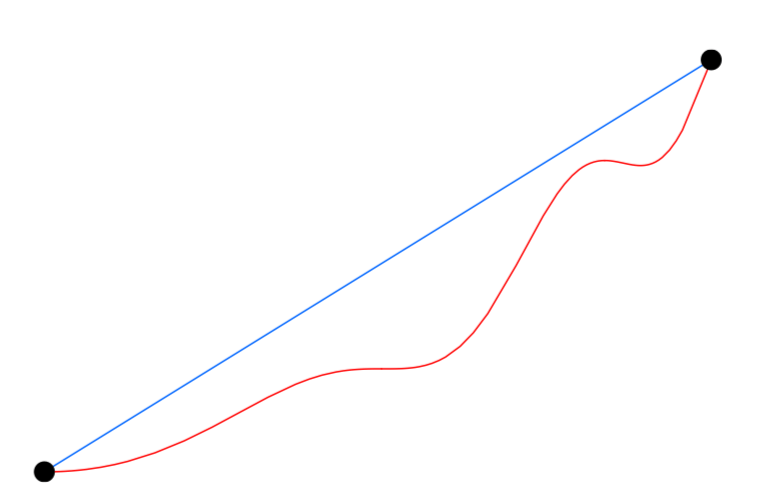
\includegraphics[width=0.5\textwidth]{Figs/a1.png}
    \caption{The Shortest Path is a Straight Line.}
    \label{fig:shortest path1}
\end{figure}
\subsection{Minimal Curves, Optics, and Geodesics}
$\bullet$ \tb{Question 1:} The minimal curve problem is to find the \tb{shortest path} between two specified locations. 

In its simplest manifestation, we are given two distinct points
\begin{align*}
\mathbf{a}=(a, \alpha) \quad \text { and } \quad \mathbf{b}=(b, \beta) \quad \text { in the plane } \mathbb{R}^{2}
\end{align*}
and our task is to find the curve of shortest length connecting them. 
\begin{rema}
"Obviously", as you learn in childhood, the shortest route between two points is a straight line. Mathematically, then, the minimizing curve should be the graph of the particular affine function 
\begin{align*}
y=c x+d=\frac{\beta-\alpha}{b-a}(x-a)+\alpha
\end{align*}
that passes through or interpolates the two points. 
\end{rema}
$\bullet$ \tb{Mathematical Formulation:} 

Assume that the minimal curve is given as the graph of a smooth function $y=u(x)$. Then, the length of the curve is given by the standard arc length integral
\begin{align}
J[u]=\int_{a}^{b} \sqrt{1+u^{\prime}(x)^{2}} d x \label{eq:odnfdaf}
\end{align}
where we abbreviate $u^{\prime}=d u / d x$. The function $u(x)$ is required to satisfy the \tb{boundary conditions}
\begin{align*}
u(a)=\alpha, \quad u(b)=\beta,
\end{align*}
in order that its graph pass through the two prescribed points. 
\begin{rema}
The minimal curve problem asks us to find the function $y=u(x)$ that minimizes the arc length functional \cref{eq:odnfdaf} in piecewise $\mathrm{C}^{1}$ function space. One of the motivating tasks of the calculus of variations, then, is to rigorously prove that our  intuition of affine function indeed correct. Note continuous functions which are not piecewise $\mathrm{C}^{1}$ need not have a well-defined arc length. 
\end{rema}
$\bullet$ \tb{{Question 2 (Fermat’s Principle):}  Light travels along the path that minimizes the travel time}

As always, Nature seeks the most economical  solution. In an \tb{inhomogeneous} planar optical medium, the speed of light, $c(x, y)$, varies from point to point, depending on the optical properties. 

$\bullet$ \tb{Mathematical Formulation:} 

Speed equals the time derivative of distance traveled, namely, the arc length of the curve $y=u(x)$ traced by the light ray. Thus,
\begin{align*}
c(x, u(x))=\frac{d s}{d t}=\sqrt{1+u^{\prime}(x)^{2}} \frac{d x}{d t} .
\end{align*}
Integrating from start to finish, we conclude that the total travel time along the curve is equal to
\begin{align*}
T[u]=\int_{0}^{T} d t=\int_{a}^{b} \frac{d t}{d x} d x=\int_{a}^{b} \frac{\sqrt{1+u^{\prime}(x)^{2}}}{c(x, u(x))} d x .
\end{align*}
Fermat's Principle states that, to get from point $\mathbf{a}=(a . \alpha)$ to point $\mathbf{b}=(b, \beta)$, the light ray follows the curve $y=u(x)$ that minimizes this functional subject to the boundary conditions
\begin{align*}
u(a)=\alpha, \quad u(b)=\beta,
\end{align*}
\begin{enumerate}
    \item If the medium is homogeneous, e.g., a vacuum,  then $c(x, y) \equiv c$ is constant, and $T[u]$ is a multiple of the arc length functional \cref{eq:odnfdaf}.
    \item In an inhomogeneous medium, the path taken by the light ray is no longer evident, and we are in need of a systematic method for solving the minimization problem.
\end{enumerate}
\begin{figure}[ht]
    \centering
    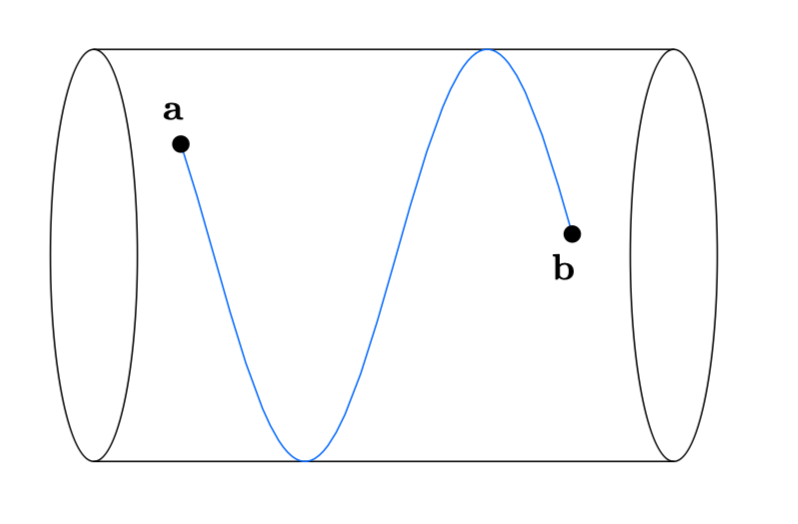
\includegraphics[width=0.5\textwidth]{Figs/a2.png}
    \caption{Geodesics on a Cylinder}
    \label{fig:shortest path2}
\end{figure}
$\bullet$ \tb{Question 3:} Find geodesics (curves of minimal length) on a curved surface.

 Given two points $\mathbf{a},\mathbf{b}$ lying on a surface $S \subset \mathbb{R}^{3}$, we seek the curve $C \subset S$ that joins them and has the minimal possible length. For example,  $S$ may a circular cylinder.

$\bullet$ \tb{Mathematical Formulation:} 

In order to mathematically formulate the geodesic minimization problem, we suppose, for simplicity, that our surface $S \subset \mathbb{R}^{3}$ is realized as the graph of a function $z=F(x, y)$. We seek the geodesic curve $C \subset S$ that joins the given points
\begin{align*}
    \mathbf{a}=(a, \alpha, F(a, \alpha)), \quad \text{and} \quad \mathbf{b}=(b, \beta, F(b, \beta)), \quad \text{lying on the surface } S.
\end{align*}
Let us assume that $C$ can be parametrized by the $x$ coordinate, in the form
\begin{align*}
y=u(x), \quad z=v(x)=F(x, u(x))
\end{align*}
where the last equation ensures that it lies in the surface $S$. In particular, this requires $a \neq b$. 

The length of the curve is supplied by the standard three-dimensional arc length integral. Thus, to find the geodesics, we must minimize the functional
\begin{align*}
\begin{aligned}
J[u] &=\int_{a}^{b} \sqrt{1+\left(\frac{d y}{d x}\right)^{2}+\left(\frac{d z}{d x}\right)^{2}} d x \\
&=\int_{a}^{b} \sqrt{1+\left(\frac{d u}{d x}\right)^{2}+\left(\frac{\partial F}{\partial x}(x, u(x))+\frac{\partial F}{\partial u}(x, u(x)) \frac{d u}{d x}\right)^{2}} d x
\end{aligned}
\end{align*}
subject to the boundary conditions $u(a)=\alpha, u(b)=\beta$. 
\subsection{Minimal Surfaces}
The minimal surface problem is a natural generalization of the minimal curve or geodesic problem. In its simplest manifestation, we are given a simple closed curve $C \subset \mathbb{R}^{3}$. 

$\bullet$ \tb{Question:} find the surface of least total area among all those whose boundary is the curve $C$. 

Thus, we seek to minimize the surface area integral
\begin{align*}
\text { area } S=\iint_{S} d S
\end{align*}
over all possible surfaces $S \subset \mathbb{R}^{3}$ with the prescribed boundary curve $\partial S=C$. 
\begin{figure}[ht]
    \centering
    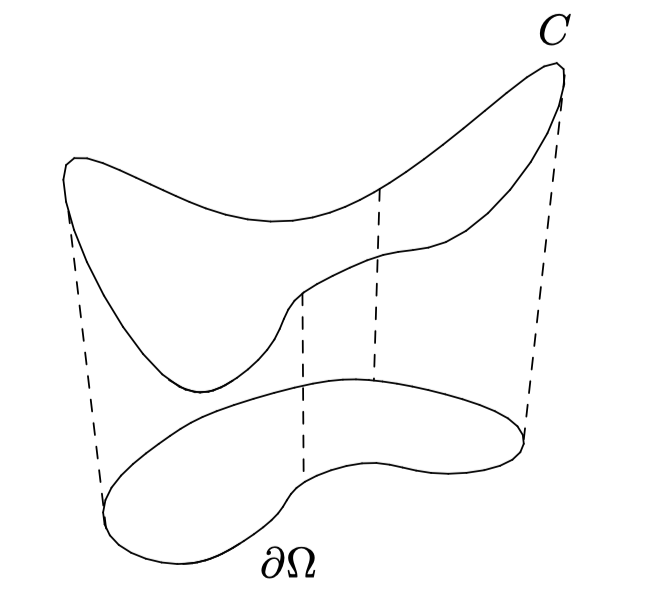
\includegraphics[width=0.3\textwidth]{Figs/a3.png}
    \caption{Minimal Surface.}
    \label{fig:Minimal Surface}
\end{figure}
\begin{exma}
For example, if $C$ is a closed plane curve, e.g., a circle, then the minimal surface will just be the planar region it encloses. But, if the curve $C$ twists into the third dimension, then the shape of the minimizing surface is by no means evident. Physically, if we bend a wire in the shape of the curve $C$ and then dip it into soapy water, the surface tension forces in the resulting soap film will cause it to minimize surface area, and hence be a minimal surface.
\end{exma}

$\bullet$ \tb{Mathematical Formulation:} 

For simplicity, we shall assume that the bounding curve $C$ projects down to a simple closed curve $\Gamma=\partial \Omega$ that bounds an open domain $\Omega \subset \mathbb{R}^{2}$ in the $(x, y)$ plane, as in \cref{fig:Minimal Surface}. The space curve $C \subset \mathbb{R}^{3}$ is then given by $z=g(x, y)$ for $(x, y) \in \Gamma=\partial \Omega$. For "reasonable" boundary curves $C$, we expect that the minimal surface $S$ will be described as the graph of a function $z=u(x, y)$ parametrized by $(x, y) \in \Omega$. According to the basic calculus, the surface area of such a graph is given by the double integral
\begin{align}
J[u]=\iint_{\Omega} \sqrt{1+\left(\frac{\partial u}{\partial x}\right)^{2}+\left(\frac{\partial u}{\partial y}\right)^{2}} d x d y\label{eq:Ldfds}
\end{align}
To find the minimal surface, then, we seek the function $z=u(x, y)$ that minimizes the surface area integral when subject to the boundary conditions
\begin{align*}
u(x, y)=g(x, y) \quad \text { for } \quad(x, y) \in \partial \Omega
\end{align*}
that prescribe the boundary curve $C$. 
As we will see later the solutions to this minimization problem satisfy a complicated nonlinear second order partial differential equation.

\begin{exma}\label{exm:aodmczcd}
A simple version of the minimal surface problem is to find minimal surfaces with rotational symmetry. A surface of revolution is obtained by revolving a plane curve about an axis, which, for definiteness, we take to be the $x$ axis. Thus, given two points $\mathbf{a}=(a, \alpha), \mathbf{b}=(b, \beta) \in \mathbb{R}^{2}$, the goal is to find the curve $y=u(x)$ joining them such that the surface of revolution obtained by revolving the curve around the $x$-axis has the least surface area. Each cross-section of the resulting surface is a circle centered on the $x$ axis. The area of such a surface of revolution is given by
\begin{align}
J[u]=\int_{a}^{b} 2 \pi|u| \sqrt{1+u^{\prime 2}} d x\label{eq:inbdf}
\end{align}
We seek a minimizer of this integral among all functions $u(x)$ that satisfy the fixed boundary conditions $u(a)=\alpha, u(b)=\beta$.
\end{exma}

\subsection{Isoperimetric Problems and Constraints}
$\bullet$ \tb{Question:} The simplest \tb{isoperimetric} problem is to construct the simple closed plane curve of a fixed length $\ell$ that encloses the domain of largest area. 

$\bullet$ \tb{Mathematical Formulation:} 

In other words, we seek to maximize area $$\text{$\Omega=\iint_{\Omega} d x d y$ subject to the constraint length $\partial \Omega=\oint_{\partial \Omega} d s=\ell$}$$
over all possible domains $\Omega \subset \mathbb{R}^{2}$. 
\begin{rema}
Of course, the "obvious" solution to this problem is that the curve must be a circle whose perimeter is $\ell$, whence the name "isoperimetric". Note that the problem, as stated, \tb{does not have a unique solution}, since if $\Omega$ is a maximizing domain, any translated or rotated version of $\Omega$ will also maximize area subject to the length constraint.
\end{rema}

$\dagger$ \tb{Variation 1:} 

To make progress on the isoperimetric problem, let us assume that the boundary curve is parametrized by its arc length, i.e. $\mathbf{x}(s)=(x(s), y(s))$ with $0 \leq s \leq \ell$, subject to the \tb{requirement} that
\begin{align}
\left(\frac{d x}{d s}\right)^{2}+\left(\frac{d y}{d s}\right)^{2}=1\label{eq:ibdadf}
\end{align}
We can compute the area of the domain by a line integral around its boundary,
\begin{align*}
\text { area } \Omega=\oint_{\partial \Omega} x d y=\int_{0}^{\ell} x \frac{d y}{d s} d s
\end{align*}
and thus we seek to maximize the latter integral subject to the arc length constraint \cref{eq:ibdadf}. We also impose \tb{periodic boundary conditions}
\begin{align*}
x(0)=x(\ell), \quad y(0)=y(\ell),
\end{align*}
that guarantee that the curve $\mathbf{x}(s)$ closes up. (Technically, we should also make sure that $\mathbf{x}(s) \neq \mathbf{x}\left(s^{\prime}\right)$ for any $0 \leq s<s^{\prime}<\ell$, ensuring that the curve does not cross itself.)

$\dagger$ \tb{Variation 2:} 
\begin{figure}[ht]
    \centering
    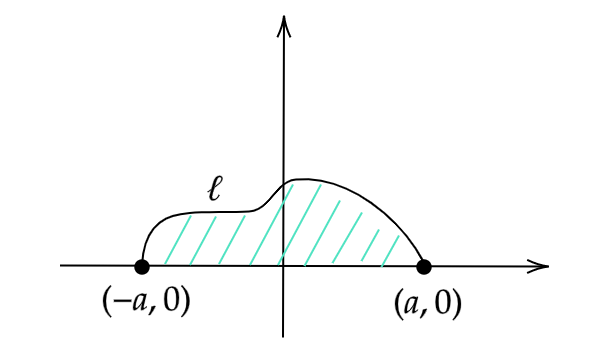
\includegraphics[width=0.5\textwidth]{Figs/a4.png}
    % \caption{Minimal Surface.}
    % \label{fig:Minimal Surface}
\end{figure}

A simpler isoperimetric problem, but one with a less evident solution, is the following. Among all curves of length $\ell$ in the upper half plane that connect two points $(-a, 0)$ and $(a, 0)$, find the one that, along with the interval $[-a, a]$, encloses the region having the largest area. Of course, we must take $\ell \geq 2 a$, as otherwise the curve will be too short to connect the points. In this case, we assume the curve is represented by the graph of a non-negative function $y=u(x)$, and we seek to maximize the functional
$$\text{$\int_{-a}^{a} u d x \quad$ subject to the constraint $\quad \int_{-a}^{a} \sqrt{1+u^{\prime 2}} d x=\ell$.}$$
\begin{rema}
In the previous formulation \cref{eq:ibdadf}, the arc length \tb{constraint was imposed at every point}, whereas here it is manifested as an \tb{integral constraint}. Such constrained variational problems can profitably be viewed as \tb{function space versions of constrained optimization problems.} Thus, not surprisingly, their analytical solution will require the introduction of suitable \tb{Lagrange multipliers.}
\end{rema}
\section{The Euler–Lagrange Equation}
Let us now discuss the most basic analytical techniques for solving such minimization problems. We will exclusively deal with classical techniques, see \cite{dacorogna2014introduction} for  more modern direct methods.

$\bullet$ \tb{Objective Functional with Fixed Endpoints}

Let us concentrate on the simplest class of variational problems, in which the unknown is a continuously differentiable scalar function, and the functional to be minimized depends upon at most its first derivative. The basic minimization problem, then, is to determine a suitable function $y=u(x) \in \mathrm{C}^{1}[a, b]$ that minimizes the \tb{objective functional}
\begin{align}
J[u]=\int_{a}^{b} L\left(x, u, u^{\prime}\right) d x \label{eq:odnmfa}
\end{align}
\begin{defa}\bfs{Lagrangian}
The integrand is known as the \tb{Lagrangian} for the variational problem. We usually assume that the Lagrangian $L(x, u, p)$ is a reasonably smooth function of all three of its (scalar) arguments $x, u$, and $p$, which represents the derivative $u^{\prime} .$
\end{defa}
\begin{exma}
For example, the arc length functional \cref{eq:odnfdaf} has Lagrangian function $L(x, u, p)=\sqrt{1+p^{2}}$, whereas in the surface of revolution problem \cref{eq:inbdf}, $L(x, u, p)=2 \pi|u| \sqrt{1+p^{2}}$. (In the latter case, the points where $u=0$ are slightly problematic, since $L$ is not continuously differentiable there.)
\end{exma}

In order to uniquely specify a minimizing function, we must impose suitable \tb{boundary conditions} at the endpoints of the interval. To begin with, we concentrate on \tb{fixed endpoints}
\begin{align}
u(a)=\alpha, \quad u(b)=\beta,\label{eq:onmccz}
\end{align}
at the two endpoints. At the end of this section, we consider \tb{other possibilities.}

\subsection{The First Variation}
As mentioned, here we would like to find potential minimizer which is called cirtial functions that will lead to $0$ gradient of the functional over infinite dimensional function space.
\begin{rema}
Of course, not every critical point turns out to be a minimum - maxima, saddles, and many degenerate points are also critical. The characterization of nondegenerate critical points as local minima or maxima relies on the second derivative test, whose functional version, known as the second variation, will be is the topic of \cref{sec:secondvar}.
\end{rema}
\subsubsection{General Definition}
Given a manifold $M$ representing (continuous/smooth) functions $\rho$ (with certain boundary conditions etc.), and a \tb{functional} $F$ defined as
\begin{align*}
F: M \rightarrow \mathbb{R} \quad \text { or } \quad F: M \rightarrow \mathbb{C}
\end{align*}
the \tb{functional derivative} of $F[\rho]$, denoted $\delta F / \delta \rho$ or $\nabla F[\rho]$, is defined through \tb{first variation}) 
\begin{align*}
\begin{aligned}
\int \frac{\delta F}{\delta \rho}(x) \phi(x) d x &=\lim _{\varepsilon \rightarrow 0} \frac{F[\rho+\varepsilon \phi]-F[\rho]}{\varepsilon} \\
&=\left[\frac{d}{d \varepsilon} F[\rho+\varepsilon \phi]\right]_{\varepsilon=0}
\end{aligned}
\end{align*}
where $\phi$ is an arbitrary function. The quantity $\varepsilon \phi$ is called the \tb{variation} of $\rho$. Note the above $dx$ may be other measures other than the Lebesgue measure (better to write it as $d\mu$).
In other words,
\begin{align*}
\phi \mapsto\left[\frac{d}{d \varepsilon} F[\rho+\varepsilon \phi]\right]_{\varepsilon=0}
\end{align*}
is a \tb{linear functional} (not always, but usually, here we assume this condition is satisfied), so one may apply the \tb{Riesz-Markov-Kakutani representation theorem} to represent this functional as integration against some measure (here we also need additional assumptions like the positive linear functional, but we omit here. So iff those conditions are satisfied, then we call the functional is differentiable).
Then $\delta F / \delta \rho$ or $\nabla F[\rho]$ is defined to be the \tb{Radon-Nikodym derivative} of this measure. In the following we may use $\langle\cdot, \cdot\rangle$ to denote the function inner product.
\begin{rema}
{In some case we could obtain an explicit formula for $\nabla F[\rho]$ w.r.t. \tb{Lebesgue measure}, while in other cases, the exact measure is not that clear.} See nex section.
\end{rema}

One thinks of the function $\delta F / \delta \rho$ as the gradient of $F$ at the point $\rho$ and the \tb{first variation}
\begin{align*}
\int \frac{\delta F}{\delta \rho}(x) \phi(x) d x
\end{align*}
as the \tb{directional derivative} at point $\rho$ in the direction of $\phi$. Then \tb{analogous to vector calculus}, the inner product with the gradient gives the \tb{directional derivative}.
\begin{rema}\bfs{comparison}
\begin{enumerate}
    \item The \tb{first variation} of the functional $F[\rho]$ is 
$$\delta F[\rho ; \phi]=\int \frac{\delta F}{\delta \rho}(x) \phi(x) d x$$
\item Heuristically, $\phi$ is the change at $\rho$ at similar to total differential of $F\left(\rho_{1}, \rho_{2}, \ldots, \rho_{n}\right)$, we have 
\begin{align*}
d F=\sum_{i=1}^{n} \frac{\partial F}{\partial \rho_{i}} d \rho_{i}
\end{align*}
where $\rho_{1}, \rho_{2}, \ldots, \rho_{n}$ are independent variables.
\end{enumerate}
Comparing the last two equations, the functional derivative $\delta F / \delta \rho(x)$ has a role similar to that of the partial derivative $\partial F / \partial \rho_{i}$, where the variable of integration $x$ is like a continuous version of the summation index $i$.
\end{rema}

\subsubsection{Special Case for Fixed Endpoints}
Directional derivative formula:
\begin{align}
\langle\nabla J[u], v\rangle=\left.\frac{d}{d \varepsilon} J[u+\varepsilon v]\right|_{\varepsilon=0}\label{eq:ondfvad}
\end{align}
\begin{rema}
Classically, $v$ is known as a variation in the function $u$, sometimes written $v=\delta u$, whence the term "calculus of variations".
\end{rema}


Now, starting with \cref{eq:odnmfa}, for each fixed $u$ and $v$, we must compute the derivative of the function
\begin{align*}
h(\varepsilon)=J[u+\varepsilon v]=\int_{a}^{b} L\left(x, u+\varepsilon v, u^{\prime}+\varepsilon v^{\prime}\right) d x
\end{align*}
Assuming sufficient smoothness of the integrand allows us to bring the derivative inside the integral and so, by the chain rule,
\begin{align*}
\begin{aligned}
h^{\prime}(\varepsilon)=\frac{d}{d \varepsilon} J[u+\varepsilon v] &=\int_{a}^{b} \frac{d}{d \varepsilon} L\left(x, u+\varepsilon v, u^{\prime}+\varepsilon v^{\prime}\right) d x \\
&=\int_{a}^{b}\left[v \frac{\partial L}{\partial u}\left(x, u+\varepsilon v, u^{\prime}+\varepsilon v^{\prime}\right)+v^{\prime} \frac{\partial L}{\partial p}\left(x, u+\varepsilon v, u^{\prime}+\varepsilon v^{\prime}\right)\right] d x
\end{aligned}
\end{align*}
Therefore, setting $\varepsilon=0$  to evaluate \cref{eq:ondfvad}, we find
\begin{align}
\langle\nabla J[u], v\rangle=\int_{a}^{b}\left[v \frac{\partial L}{\partial u}\left(x, u, u^{\prime}\right)+v^{\prime} \frac{\partial L}{\partial p}\left(x, u, u^{\prime}\right)\right] d x \label{eq:opdncdf}
\end{align}
The resulting integral is \tb{first variation} of the functional $J[u]$. 

The condition
\begin{align*}
\langle\nabla J[u], v\rangle=0
\end{align*}
for a minimizer is known as the \tb{weak form of the variational principle}.


$\bullet$ \tb{Explicit Formula} for $\nabla J[u]$:

To obtain an explicit formula for $\nabla J[u]$ w.r.t. \tb{Lebesgue measure}, the right hand side of \cref{eq:ondfvad} needs to be written as an inner product,
\begin{align*}
\langle\nabla J[u], v\rangle=\int_{a}^{b} \nabla J[u] v d x=\int_{a}^{b} h v d x
\end{align*}
between some function $h(x)=\nabla J[u]$ and the variation $v$. The first summand has this form, but the derivative $v^{\prime}$ appearing in the second summand is problematic. We use \tb{integration by parts}. If we set
\begin{align*}
r(x) \equiv \frac{\partial L}{\partial p}\left(x, u(x), u^{\prime}(x)\right)
\end{align*}
we can rewrite the second  term in \cref{eq:opdncdf} as
\begin{align}
\int_{a}^{b} r(x) v^{\prime}(x) d x=[r(b) v(b)-r(a) v(a)]-\int_{a}^{b} r^{\prime}(x) v(x) d x\label{eq:jdncdaf}
\end{align}
where, again by the chain rule,
\begin{align*}
r^{\prime}(x)=\frac{d}{d x}\left(\frac{\partial L}{\partial p}\left(x, u, u^{\prime}\right)\right)=\frac{\partial^{2} L}{\partial x \partial p}\left(x, u, u^{\prime}\right)+u^{\prime} \frac{\partial^{2} L}{\partial u \partial p}\left(x, u, u^{\prime}\right)+u^{\prime \prime} \frac{\partial^{2} L}{\partial p^{2}}\left(x, u, u^{\prime}\right) .
\end{align*}
So far we have not imposed any conditions on our variation $v(x)$. We are only comparing the values of $J[u]$ among functions that satisfy the imposed \tb{boundary conditions} \cref{eq:onmccz}. Therefore, we must make sure that the varied function
\begin{align*}
\widehat{u}(x)=u(x)+\varepsilon v(x)
\end{align*}
remains within this set of functions, and so
\begin{align*}
\widehat{u}(a)=u(a)+\varepsilon v(a)=\alpha, \quad \widehat{u}(b)=u(b)+\varepsilon v(b)=\beta .
\end{align*}
For this to hold, the variation $v(x)$ must satisfy the corresponding \tb{homogeneous boundary conditions}
\begin{align*}
v(a)=0, \quad v(b)=0 .
\end{align*}
As a result, both boundary terms in our integration by parts formula \cref{eq:jdncdaf} vanish, and we can write \cref{eq:opdncdf} as
\begin{align}
\langle\nabla J[u], v\rangle=\int_{a}^{b} \nabla J[u] v d x=\int_{a}^{b} v\left[\frac{\partial L}{\partial u}\left(x, u, u^{\prime}\right)-\frac{d}{d x}\left(\frac{\partial L}{\partial p}\left(x, u, u^{\prime}\right)\right)\right] d x.
\end{align}
Since this holds for all variations $v(x)$, we conclude that 
\begin{align}
\nabla J[u]=\frac{\partial L}{\partial u}\left(x, u, u^{\prime}\right)-\frac{d}{d x}\left(\frac{\partial L}{\partial p}\left(x, u, u^{\prime}\right)\right) .\label{eq:oidnfdaf}
\end{align}
This is our \tb{explicit formula} for the functional gradient or variational derivative of the functional \cref{eq:odnmfa} with Lagrangian $L(x,u,p)$. Observe that the gradient $\nabla J[u]$ of a functional is a function.

\subsubsection{Euler-Lagrange Equation}
\begin{defa}\bfs{Critical Functions}
The \tb{critical functions} $u(x)$ are, by definition, those for which the functional gradient vanishes: $\nabla J[u]=0$.
\end{defa}
\begin{rema}
Please also see \cref{lem:fund1} and \cref{lem:fund2}. In explicit formula, the minimum lead to the requirement of critical functions.
\end{rema}
 Thus, critical $u(x)$ must satisfy the \tb{Euler-Lagrange equation}:
\begin{align}
\nabla J[u]=\frac{\partial L}{\partial u}\left(x, u, u^{\prime}\right)-\frac{d}{d x} \frac{\partial L}{\partial p}\left(x, u, u^{\prime}\right)=0\label{eq:ndcdfadf}
\end{align}

% $\bullet$ \tb{Special case with fixed boundary condition:}
In view of \cref{eq:oidnfdaf} the critical equation is a \tb{second order ordinary differential equation}:
\begin{align}
E\left(x, u, u^{\prime}, u^{\prime \prime}\right)=\frac{\partial L}{\partial u}\left(x, u, u^{\prime}\right)-\frac{\partial^{2} L}{\partial x \partial p}\left(x, u, u^{\prime}\right)-u^{\prime} \frac{\partial^{2} L}{\partial u \partial p}\left(x, u, u^{\prime}\right)-u^{\prime \prime} \frac{\partial^{2} L}{\partial p^{2}}\left(x, u, u^{\prime}\right)=0,\label{eq:dnfnadfdf}
\end{align}
known as the {Euler-Lagrange equation} associated with the variational problem \cref{eq:odnmfa}.
\begin{rema} \label{re:lccz} In \tb{ general  case} without no explicit formula of $\nabla J[u]$ (e.g. without fixed boundary conditions), we should consider directly \tb{enforce
\cref{eq:opdncdf} to be $0$ for all $v$.}
\end{rema}
\begin{thma}
Suppose the Lagrangian function is at least twice continuously differentiable: $L(x, u, p) \in \mathrm{C}^{2}$. Then any $\mathrm{C}^{2}$ minimizer $u(x)$ to the corresponding functional $J[u]=\int_{a}^{b} L\left(x, u, u^{\prime}\right) d x$, subject to the selected boundary conditions, must satisfy the associated Euler-Lagrange equation \cref{eq:ndcdfadf}.
\end{thma}
\begin{proof}
It is easy to understand that the continuously differentiable and minimum will lead to the weak form of the variational principle $\langle\nabla J[u], v\rangle=0$ (even there is no explicit form of $J[u]$). Since other wise we may move the $u$ a little bit in some direction of $v$ and get a smaller value. From \cref{lem:fund1} and \cref{lem:fund2}, in explicit formula, the minimum lead to the requirement of critical functions, and therefore we have condition \cref{eq:ndcdfadf}.
\end{proof}
\subsection{Examples}
\subsubsection{Curves of Shortest Length - Planar Geodesics}\label{sec:planargeo}
$\bullet$ \tb{Objective:}

Finding the curve of shortest length connecting two points $\mathbf{a}=(a, \alpha), \quad \mathbf{b}=(b, \beta) \in \mathbb{R}^{2}$ in the plane is to minimize:
$$\text{$J[u]=\int_{a}^{b} \sqrt{1+u^{\prime 2}} d x \quad$ with Lagrangian $\quad L(x, u, p)=\sqrt{1+p^{2}}$}$$
subject to the \tb{boundary conditions}
\begin{align*}
u(a)=\alpha, \quad u(b)=\beta .
\end{align*}

$\bullet$ \tb{Solution:}

Since
\begin{align*}
\frac{\partial L}{\partial u}=0, \quad \frac{\partial L}{\partial p}=\frac{p}{\sqrt{1+p^{2}}}
\end{align*}
the Euler-Lagrange equation \cref{eq:dnfnadfdf} in this case takes the form
\begin{align*}
0=-\frac{d}{d x} \frac{u^{\prime}}{\sqrt{1+u^{\prime 2}}}=-\frac{u^{\prime \prime}}{\left(1+u^{\prime 2}\right)^{3 / 2}}
\end{align*}
Since the denominator does not vanish, this is the same as the simplest second order ordinary differential equation
\begin{align}
u^{\prime \prime}=0 \label{eq:ccdf}
\end{align}
We deduce that the solutions to the Euler-Lagrange equation are all affine functions, $u=c x+d$, whose graphs are straight lines. Since our solution must also satisfy the boundary conditions, the only critical function - and hence the sole candidate for a minimizer - is the straight line
\begin{align*}
y=\frac{\beta-\alpha}{b-a}(x-a)+\alpha
\end{align*}
passing through the two points. Thus, the Euler-Lagrange equation helps to reconfirm our intuition that straight lines minimize distance.
\begin{rema}
A function satisfies the Euler-Lagrange equation and the boundary conditions merely confirms its status as a critical function, and does not guarantee that it is the minimizer. Indeed, any critical function is also a candidate for maximizing the variational problem, too.
\end{rema}
\subsubsection{The Brachistochrone Problem}
The most famous classical variational principle is the so-called brachistochrone problem. An experimenter lets a bead slide down a wire that connects two fixed points under the influence of gravity. The goal is to shape the wire in such a way that, starting from rest, the bead slides from one end to the other \tb{in minimal time}.

$\bullet$ \tb{Math Formulation:}

We take, without loss of generality, the starting point of the bead to be at the origin: $\mathbf{a}=(0,0)$. The wire will bend downwards, and so, to avoid distracting minus signs in the subsequent formulae, we take the vertical $y$ axis to point downwards. The shape of the wire will be given by the graph of a function $y=u(x) \geq 0$. The end point $\mathbf{b}=(b, \beta)$ is assumed to lie below and to the right, and so $b>0$ and $\beta>0$.
\begin{figure}[ht]
    \centering
    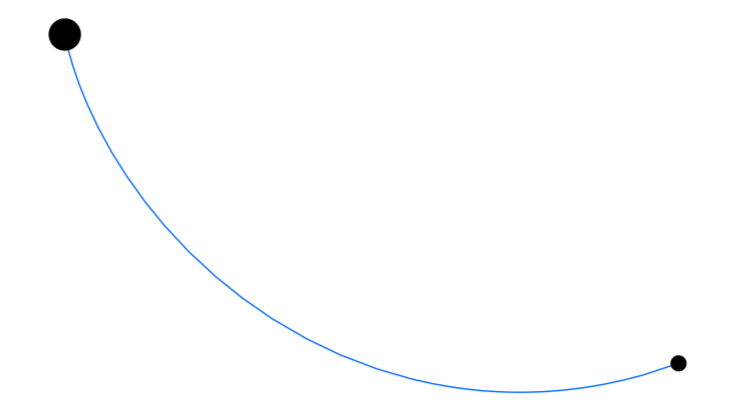
\includegraphics[width=0.5\textwidth]{Figs/a5.png}
    \caption{The Brachistochrone Problem.}
    % \label{fig:Minimal Surface}
\end{figure}
To mathematically formulate the problem, the first step is to find the formula for the transit time of the bead sliding along the wire. If $v(x)$ denotes the instantaneous speed of descent of the bead when it reaches position $(x, u(x))$, then the total travel time is
\begin{align}
T[u]=\int_{0}^{\ell} \frac{d s}{v}=\int_{0}^{b} \frac{\sqrt{1+u^{\prime 2}}}{v} d x\label{eq:udjbcadf}
\end{align}
where $d s=\sqrt{1+u^{\prime 2}} d x$ is the usual arc length element, and $\ell$ is the overall length of the wire.
\begin{rema}\bfs{conservation of energy }
We shall use conservation of energy to determine a formula for the speed $v$ as a function of the position along the wire. The kinetic energy of the bead is $\frac{1}{2} m v^{2}$, where $m$ is its mass. On the other hand, due to our sign convention, the potential energy of the bead when it is at height $y=u(x)$ is $-m g u(x)$, where $g$ the gravitational constant, and we take the initial height as the zero potential energy level. The bead is initially at rest, with 0 kinetic energy and 0 potential energy. Assuming that frictional forces are negligible, conservation of energy implies that the total energy must remain equal to $0$ , and hence
\begin{align*}
0=\frac{1}{2} m v^{2}-m g u
\end{align*}
We can solve this equation to determine the bead's speed as a function of its height: \begin{align*} v=\sqrt{2 g u}. \end{align*}
\end{rema}
 Substituting above expression into\cref{eq:udjbcadf}, we conclude that the shape $y = u(x)$ of the wire is obtained by minimizing the functional is obtained by minimizing the functional
\begin{align*}
T[u]=\int_{0}^{b} \sqrt{\frac{1+u^{\prime 2}}{2 g u}} d x
\end{align*}
\tb{subject to the boundary conditions}
\begin{align*}
u(0)=0, \quad u(b)=\beta .
\end{align*}
The associated \tb{Lagrangian} is 
\begin{align}
L(x, u, p)=\sqrt{\frac{1+p^{2}}{u}}\label{eq:fdadyrtrq}
\end{align}
where we omit an irrelevant factor of $\sqrt{2 g}$ (or adopt physical units in which $g=\frac{1}{2}$). We compute
\begin{align*}
\frac{\partial L}{\partial u}=-\frac{\sqrt{1+p^{2}}}{2 u^{3 / 2}}, \quad \frac{\partial L}{\partial p}=\frac{p}{\sqrt{u\left(1+p^{2}\right)}}
\end{align*}
Therefore, the \tb{Euler-Lagrange equation} for the brachistochrone functional is
\begin{align*}
-\frac{\sqrt{1+u^{\prime 2}}}{2 u^{3 / 2}}-\frac{d}{d x} \frac{u^{\prime}}{\sqrt{u\left(1+u^{\prime 2}\right)}}=-\frac{2 u u^{\prime \prime}+u^{\prime 2}+1}{2 \sqrt{u\left(1+u^{\prime 2}\right)}}=0
\end{align*}
Thus, the minimizing functions solve the \tb{nonlinear second order ordinary differential equation}:
\begin{align*}
2 u u^{\prime \prime}+u^{\prime 2}+1=0
\end{align*}

Rather than try to solve this differential equation directly, we note that the Lagrangian does not depend upon $x$, and therefore we can appeal to the following result.
\paragraph{Hamiltonian Function}
We are not familiar with the second-order autonomous ode. We next show how to use Hamiltonian function to convert the above question to first-order equation.
\begin{thma}
Suppose the Lagrangian $L(x, u, p)=L(u, p)$ does not depend on $x$. Then the \tb{Hamiltonian function}
\begin{align}
H(u, p)=L(u, p)-p \frac{\partial L}{\partial p}(u, p)\label{eq:doncdadf}
\end{align}
is a \tb{first integral for the Euler-Lagrange equation}, meaning that it is constant on each solution:
\begin{align}
H\left(u(x), u^{\prime}(x)\right)=c\label{eq:xcadfda}
\end{align}
for some $c \in \mathbb{R}$, whose value can depend upon the solution $u(x)$.
\end{thma}
\begin{proof}
Differentiating \cref{eq:doncdadf}, we find
\begin{align*}
\frac{d}{d x} H\left(u, u^{\prime}\right)=\frac{d}{d x}\left[L\left(u, u^{\prime}\right)-u^{\prime} \frac{\partial L}{\partial p}\left(u, u^{\prime}\right)\right]=u^{\prime}\left(\frac{\partial L}{\partial u}\left(u, u^{\prime}\right)-\frac{d}{d x} \frac{\partial L}{\partial p}\left(u, u^{\prime}\right)\right)=0,
\end{align*}
This implies that the Hamiltonian function is constant on solution of Euler-Lagrange equation \cref{eq:ndcdfadf}, thereby establishing the conclusion.
\end{proof}
\begin{rema}\bfs{how to solve first order autonomous equation?}
\cref{eq:doncdadf} has the form of an implicitly defined first order ordinary differential equation which can, in fact, be integrated. Indeed, solving for
\begin{align*}
u^{\prime}=h(u, c)
\end{align*}
produces an autonomous first order differential equation, whose general solution can be obtained by \tb{integration}:
\begin{align*}
\int \frac{d u}{h(u, c)}=x+\delta
\end{align*}
where $\delta$ is a second integration constant.
\end{rema}
\paragraph{Solve the Brachistochrone Problem}
In our case \cref{eq:fdadyrtrq}, the Hamiltonian function is
\begin{align*}
H(u, p)=L-p \frac{\partial L}{\partial p}=\frac{1}{\sqrt{u\left(1+p^{2}\right)}}
\end{align*}
Thus, we have
$H\left(x, u, u^{\prime}\right)=\frac{1}{\sqrt{u\left(1+u^{\prime 2}\right)}}=c$,  which we rewrite as $u\left(1+u^{\prime 2}\right)=k$,
where $k=1 / c^{2}$ is a constant. Solving for the derivative $u^{\prime}$ results in the first order autonomous ordinary differential equation
\begin{align*}
\frac{d u}{d x}=\sqrt{\frac{k-u}{u}}
\end{align*}
This equation can be explicitly solved by separation of variables, and so
\begin{align*}
\int \sqrt{\frac{u}{k-u}} d u=x+\delta
\end{align*}
for some constant $\delta$. The left hand integration relies on the trigonometric substitution
\begin{align*}
u=\frac{1}{2} k(1-\cos \theta)
\end{align*}
whereby
\begin{align*}
x+\delta=\frac{k}{2} \int \sqrt{\frac{1-\cos \theta}{1+\cos \theta}} \sin \theta d \theta=\frac{k}{2} \int(1-\cos \theta) d \theta=\frac{1}{2} k(\theta-\sin \theta)
\end{align*}
The left hand boundary condition implies $\delta=0$ (recall we start from $\mathbf{a}=(0,0)$), and so the solution to the Euler-Lagrange equation are curves parametrized by
\begin{align}
x=r(\theta-\sin \theta), \quad u=r(1-\cos \theta) .\label{eq:dflmczc}
\end{align}
With a little more work, it can be proved that the parameter $r=\frac{1}{2} k$ is uniquely determined by the right hand boundary condition, and moreover, the resulting curve supplies the global minimizer of the brachistochrone functional.

The parametrized curve \cref{eq:dflmczc} is known as a cycloid, which can be visualized as the curve traced by a point sitting on the edge of a rolling wheel of radius $r$, as plotted in \cref{fig:Brachistochrone}. Interestingly, in certain configurations, namely if $\beta<2 b / \pi$, the cycloid that solves the brachistochrone problem dips below the right hand endpoint $\mathbf{b}=(b, \beta)$, and so the bead is moving upwards when it reaches the end of the wire.
\begin{figure}[ht]
    \centering
    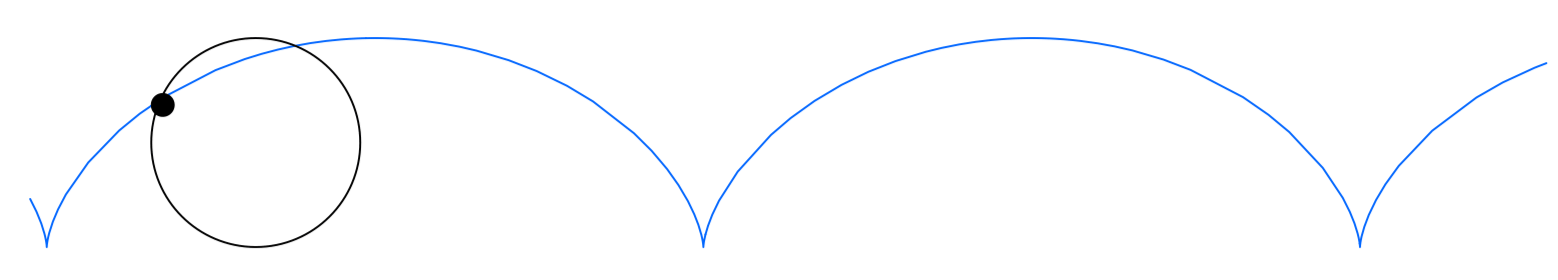
\includegraphics[width=0.6\textwidth]{Figs/a6.png}
    \caption{The Brachistochrone Problem.}
    \label{fig:Brachistochrone}
\end{figure}
\subsubsection{Minimal Surface of Revolution}
Consider \cref{exm:aodmczcd} of finding the curve connecting two points that generates a surface of revolution of minimal surface area . For simplicity, we assume that the curve is given by the graph of a non-negative function $y=u(x) \geq 0$. According to \cref{eq:inbdf}, the required curve will minimize the functional 
\begin{align}
    J[u]=\int_{a}^{b} u \sqrt{1+u^{\prime 2}} d x, \quad\text{ with Lagrangian }\quad L(x, u, p)=u \sqrt{1+p^{2}},\label{eq:omcmdadf}
\end{align}
where we have omitted an irrelevant factor of $2 \pi$ and used positivity to delete the absolute value on $u$ in the integrand.
We have
\begin{align*}
\frac{\partial L}{\partial u}=\sqrt{1+p^{2}}, \quad \frac{\partial L}{\partial p}=\frac{u p}{\sqrt{1+p^{2}}}
\end{align*}
and so the Euler-Lagrange equation is
\begin{align}
\sqrt{1+u^{\prime 2}}-\frac{d}{d x} \frac{u u^{\prime}}{\sqrt{1+u^{\prime 2}}}=\frac{1+u^{\prime 2}-u u^{\prime \prime}}{\left(1+u^{\prime 2}\right)^{3 / 2}}=0\label{eq:omcsdadfad}
\end{align}
Since the Lagrangian \cref{eq:omcmdadf} does not depend upon $x$, we can again apply Hamiltonian function:
\begin{align*}
H(u, p)=L-p \frac{\partial L}{\partial p}=\frac{u}{\sqrt{1+p^{2}}}
\end{align*}
and hence \cref{eq:xcadfda} implies $H\left(u, u^{\prime}\right)=\frac{u}{\sqrt{1+u^{\prime 2}}}=c$ for some constant $c \in \mathbb{R}$. Solving for
\begin{align*}
\frac{d u}{d x}=u^{\prime}=\frac{\sqrt{u^{2}-c^{2}}}{c}
\end{align*}
results in an autonomous first order ordinary differential equation, which we can immediately solve:
\begin{align*}
\int \frac{c d u}{\sqrt{u^{2}-c^{2}}}=x+\delta
\end{align*}
where $\delta$ is a constant of integration. The most useful form of the left hand integral is in terms of the inverse to the hyperbolic cosine function $\cosh z=\frac{1}{2}\left(e^{z}+e^{-z}\right)$, whereby
\begin{align}
     \cosh ^{-1} \frac{u}{c}=x+\delta, \quad\text{ and hence }\quad u=c \cosh \left(\frac{x+\delta}{c}\right).\label{eq:cczxc}
\end{align}
In this manner, we have produced the general solution to the Euler-Lagrange equation \cref{eq:omcsdadfad}. Any solution that also \tb{satisfies the boundary conditions} provides a critical function for the surface area functional \cref{eq:omcmdadf}, and hence is a candidate for the minimizer.

$\bullet$ \tb{more discussion of  boundary conditions}

So far, we have not taken into account the boundary conditions. It turns out that there are three distinct possibilities, depending upon the configuration of the boundary points:
\begin{enumerate}
    \item There is precisely one value of the two integration constants $c, \delta$ that satisfies the two boundary conditions.
    \item There are two different possible values of $c, \delta$ that satisfy the boundary conditions.
    \item There are no values of $c, \delta$ that allow \cref{eq:cczxc} to satisfy the two boundary conditions. This occurs when the two boundary points $\mathbf{a}, \mathbf{b}$ are relatively far apart.
\end{enumerate}

In the third configuration, the physical soap film spanning the two circular wires breaks apart into two circular disks, and this defines the minimizer for the problem; there is no surface of revolution that has a smaller surface area than the two disks. However, the function that minimizes this configuration consists of two vertical lines from the boundary points to the $x$ axis, along with that segment on the axis lying between them. More precisely, we can approximate this function by a sequence of genuine functions that give progressively smaller and smaller values to the surface area functional, but \tb{the actual minimum is not attained among the class of (smooth) functions.}

There are further subtleties in the other two cases, which were completely resolved only relatively recently and is  complicated. There is an cut catenary named MacNeish frontier that determine  whether the above two-disk solution is the minimum one.

\subsubsection{The Fundamental Lemma}
The justification that a critical function satisfies the Euler-Lagrange equation relies on what is know as the Fundamental Lemma. The simplest version of this key result can be stated as follows.
\begin{lema}\label{lem:fund1}
If $f(x)$ is continuous on the closed interval $[a, b]$, and
\begin{align*}
\int_{a}^{b} f(x) v(x) d x=0
\end{align*}
for every continuous function $v(x)$, then $f(x) \equiv 0$ for all $a \leq x \leq b .$
\end{lema}
\begin{proof}
A simple proof of the stated result proceeds by setting $v(x)=f(x) .$ Then
\begin{align*}
0=\int_{a}^{b} f(x) v(x) d x=\int_{a}^{b}[f(x)]^{2} d x
\end{align*}
which, by continuity, is only possible when $f(x) \equiv 0$.
However, for many purposes, we would like to impose additional conditions on the functions $v(x)$ like smoothness, and the preceding proof will not work unless $f(x)$ satisfies the same conditions. A proof that has much wider applicability proceeds as follows. Suppose $f\left(x_{0}\right) \neq 0$ for some $a<x_{0}<b$. By replacing $f(x)$ by $-f(x)$ if necessary, we can assume $f\left(x_{0}\right)>0$. Then, by continuity, $f(x)>0$ for all $x$ lying in in some small interval around $x_{0}$, of the form $a<x_{0}-\varepsilon<x<x_{0}+\varepsilon<b$ for some $\varepsilon>0$. Choose $v(x)$ to be a continuous (with possible other conditions) function that is $>0$ in this interval and $=0$ outside. An example is the piecewise linear function
\begin{align*}
v(x)= \begin{cases}\varepsilon-\left|x-x_{0}\right|, & \left|x-x_{0}\right|<\varepsilon \\ 0, & \text { otherwise .}\end{cases}
\end{align*}
Then $f(x) v(x) \geq 0$ everywhere, hence $\int_{a}^{b} f(x) v(x) d x \geq 0$, and, by continuity, is equal to zero if and only if $f(x) v(x) \equiv 0$, which is a contradiction.
\end{proof} 
 We also have a useful strengthening:
\begin{lema}\label{lem:fund2}
If $f(x)$ is continuous on $[a, b]$, and $\int_{a}^{b} f(x) v(x) d x=0$ for every $\mathrm{C}^{\infty}$ function $v(x)$ with compact support in $(a, b)$, then $f(x) \equiv 0$ for all $a \leq x \leq b .$
\end{lema} 
\begin{proof}
Just use the smooth bump function
\begin{align*}
v(x)= \begin{cases}\varepsilon \exp \left[1-\left(\varepsilon^{-2}\left(x-x_{0}\right)^{2}-1\right)^{-2}\right], & \left|x-x_{0}\right|<\varepsilon \\ 0, & \text { otherwise }\end{cases}
\end{align*}
which, in addition to being positive on the required interval, is $\mathrm{C}^{\infty}$ everywhere, including at $x=x_{0} \pm \varepsilon$. Also note all its derivatives vanish outside the interval.
\end{proof}
Note that the condition that $v(x)$ has compact support implies that $v(a)=v(b)=0$ thus justifying our derivation of the Euler-Lagrange equation \cref{eq:ndcdfadf}.
\subsubsection{A Cautionary Example}
While the Euler-Lagrange equation is fundamental in the analysis of variational problems, it does have limitations and analysis based solely thereon may miss important features. One complicating factor is that convergence in infinite-dimensional function space is considerably more subtle than in finite-dimensional Euclidean space. So let us conclude this section with one of a large variety of cautionary examples.

Consider the problem of minimizing the integral
\begin{align}
J[u]=\int_{0}^{1}\left[\frac{1}{2}\left(u^{\prime 2}-1\right)^{2}+\frac{1}{2} u^{2}\right] d x
\end{align}
subject to the boundary conditions $u(0)=u(1)=0$. The Euler-Lagrange equation is
\begin{align}
0=-\frac{d}{d x}\left[2 u^{\prime}\left(u^{\prime 2}-1\right)\right]+u=\left(2-6 u^{\prime 2}\right) u^{\prime \prime}+u=0
\end{align}
Since the Lagrangian is independent of $x$, Hamiltonian function can be applied to reduce this to the first order ordinary differential equation:
\begin{align*}
H\left(u, u^{\prime}\right)=L\left(u, u^{\prime}\right)-u^{\prime} \frac{\partial L}{\partial p}\left(u, u^{\prime}\right)=-\frac{3}{2} u^{\prime 4}+u^{\prime 2}+\frac{1}{2}+\frac{1}{2} u^{2}=c
\end{align*}
where $c \in \mathbb{R}$. The resulting quartic polynomial in $u^{\prime}$ can be solved for $u^{\prime}=h(u, c)$, and the final autonomous first order ordinary differential equation can then be integrated. However, the resulting very complicated formula for the solution $u(x)$ is not particularly helpful, especially when one tries to impose the admitted boundary conditions to fix the values of the integration constants $c, \delta$. A numerical approximation to the preceding two point boundary value problem would be considerably more enlightening.
\begin{figure}[ht]
    \centering
    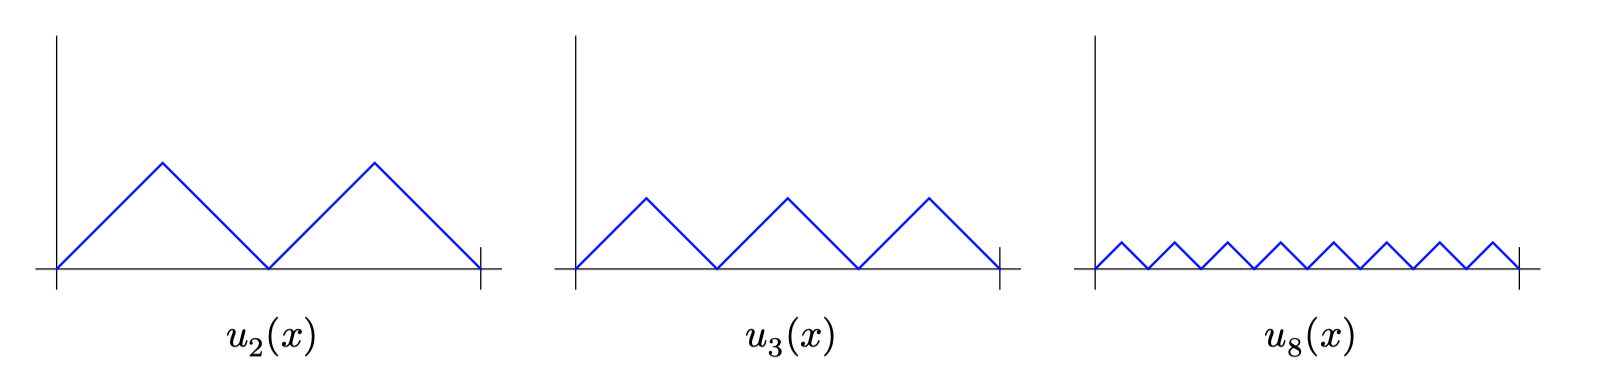
\includegraphics[width=0.7\textwidth]{Figs/a7.png}
    \caption{Sawtooth Functions. If we require $\mathrm{C}^{\infty}$ function, the smootheness of the corner is not difficult.}
    \label{fig:Sawtooth}
\end{figure}

Moreover, \tb{the solution to the Euler-Lagrange equation does not, in fact minimize  the functional,} as the following direct analysis shows. Observe that the functional is clearly bounded below by $0 \leq J[u]$. However this minimum value \tb{cannot be achieved}, since it would simultaneously require that $u^{\prime}(x)=\pm 1$ and $u(x)=0 .$ On the other hand, one can come arbitrarily close to the minimum as follows. Consider the "sawtooth" functions
\begin{align*}
u_{n}(x)=\left\{\begin{array}{ll}
x-\frac{k}{n}, & \frac{k}{n} \leq x \leq \frac{2 k+1}{2 n}, \\
\frac{k+1}{n}-x, & \frac{2 k+1}{2 n} \leq x \leq \frac{k+1}{n},
\end{array} \quad k=0, \ldots, n-1\right.
\end{align*}
which are continuous, piecewise linear, with slope $\pm 1$, three of which are plotted in  \cref{fig:Sawtooth}. For these fuctions, the first term in the integrand vanishes, and hence
\begin{align*}
J\left[u_{n}\right]=\int_{0}^{1} \frac{1}{2} u_{n}(x)^{2} d x=\sum_{j=0}^{2 n-1} \int_{j /(2 n)}^{(j+1) /(2 n)} \frac{1}{2} u_{n}(x)^{2} d x=\frac{2 n}{8 n^{2}}=\frac{1}{4 n}
\end{align*}
Thus, as $n \rightarrow \infty$, the value of $J\left[u_{n}\right] \rightarrow 0 .$ On the other hand, the uniformly to the zero function: $u_{n}(x) \rightarrow u_{*}(x) \equiv 0$, and $J\left[u_{*}\right]=\frac{1}{2}$. In other words, 
\begin{align*} \lim _{n \rightarrow \infty} J\left[u_{n}\right]=0 \neq \frac{1}{2}=J\left[\lim _{n \rightarrow \infty} u_{n}\right] . \end{align*}
We conclude that one can find functions $u(x)$ for which the value of the integral Sawtooth function is arbitrarily close to its overall minimum, but there is no function which achieves the value $J[u]=0$.
\begin{rema}
See also \cref{exm:fdafadf} for another example of no arbitrarily close to the minimum but no function can achieve.
\end{rema}

\section{Boundary Conditions.}
\subsection{Both Fixed  Endpoints}
So far, we have only imposed fixed boundary conditions on the variational problem, in which the values of the minimizer are specified at the ends of the interval.  This is exactly what we have considered in \cref{eq:onmccz}.
\subsection{Natural Boundary Conditions}
A second common type of condition is that of a free boundary, in which no conditions are imposed on the minimizer at one or both ends of the interval.
\begin{exma}Two cases in planar geodesic problem:
\begin{enumerate}
    \item One Fixed Endpoint: Consider the planar geodesic problem in which one wishes to find the curve of shortest length that connects a given point to a vertical line. That means the minimizing function is required to pass through the point $(a, \alpha)$, so that $u(a)=\alpha$, but there are no conditions at the endpoint $x=b$. Thus we are seeking the shortest curve that goes from $(a, \alpha)$ to any point on the vertical line $L_{b}=\{x=b\} .$ The minimizing curve is a horizontal straight line, so $u(x) \equiv \alpha$ for all $a \leq x \leq b$, that meets the vertical line $L_{b}$ in a perpendicular direction. 
    \item Two Fixed Endpoints: If we also impose no conditions at the initial endpoint, we then seek a curve of minimal length that goes from the vertical line $L_{a}=\{x=a\}$ to the vertical line $L_{b}=\{x=b\} .$ In this case any horizontal line will serve as a minimizer, and so the minimizer is not unique.
\end{enumerate}
\end{exma}
\begin{exma}\label{exm:bra}
In the brachistochrone problem with a free end, to determine the shape of a wire starting at the origin with the property that a bead sliding along it reaches the line $L_{b}$ in the shortest possible time, without any need to specify which point on the line it ends up on. 
\end{exma}

To analyze such problems, let us return to our general variational calculation. We need recall \cref{re:lccz} in which we mentioned we need to directly use the first variation form \cref{eq:opdncdf} where {explicit Formula} for $\nabla J[u]$ may not exist. 

$\bullet$ \tb{Objective functional:}
\begin{align*}
\min_{u} J[u]=\int_{a}^{b} L\left(x, u, u^{\prime}\right) d x
\end{align*}
where $u(x)$ is sufficiently smooth function defined for $a \leq x \leq b$.

$\bullet$ \tb{One Fixed Endpoint:}
\begin{align}
u(a)=\alpha, \label{eq:fixed_a}
\end{align}
while the value $u(b)$ at the other end of the interval \tb{remains arbitrary.}

The variation $v(x)$ must vanish at the left hand boundary point: $v(a)=0 .$ However, there are no conditions imposed on $v(b)$ at the right hand end. From  \cref{eq:opdncdf,eq:jdncdaf}, we have \tb{for any $v$}
\begin{align}
\begin{aligned}
0 &=\langle\nabla J[u], v\rangle \\
&=v(b) \frac{\partial L}{\partial p}\left(b, u(b), u^{\prime}(b)\right)+\int_{a}^{b} v\left[\frac{\partial L}{\partial u}\left(x, u, u^{\prime}\right)-\frac{d}{d x}\left(\frac{\partial L}{\partial p}\left(x, u, u^{\prime}\right)\right)\right] d x \label{eq:dfadcyc}
\end{aligned}
\end{align}
Thus, we can no longer identify the gradient of the functional $J[u]$ as the function given by the Euler-Lagrange expression, since there is an additional boundary component. Instead, let us work with \cref{eq:dfadcyc} directly. 

Since we can select any $v$, if we set $v(b)=0$, then by the same argument based on \cref{lem:fund2},  \cref{eq:dfadcyc} reduce to that that $u(x)$ must continue to satisfy the Euler-Lagrange equation. Since we can then select any $v(x)$, the term multiplying $v(b)$ must also vanish, and we conclude that the minimizing function must satisfy
\begin{align}
\frac{\partial L}{\partial p}\left(b, u(b), u^{\prime}(b)\right)=0\label{eq:dcfdfaf1}
\end{align}
This is known as a \tb{natural boundary condition}, which imposes a constraint on the minimizer at the free boundary.

$\bullet$ \tb{No Fixed Endpoints:}

The same argument implies that the minimizer must \tb{also} satisfy a natural boundary condition there:
\begin{align}
\frac{\partial L}{\partial p}\left(a, u(a), u^{\prime}(a)\right)=0\label{eq:dcfdfaf2}
\end{align}

Thus, any minimizer of the free variational problem must solve the Euler-Lagrange equation along with the \tb{two natural boundary conditions \cref{eq:dcfdfaf1} and \cref{eq:dcfdfaf2}}. 

$\bullet$ \tb{Conclusion:}
At each endpoint of the interval, any critical function of a functional, including minimizers and maximizers, must satisfy either homogeneous or inhomogeneous fixed boundary conditions, or homogeneous natural boundary conditions.
\begin{enumerate}
    \item Both Fixed  Endpoints: Euler-Lagrange equation with two fixed points.
    \item One Fixed Endpoint: Euler-Lagrange equation  with \cref{eq:fixed_a} and \cref{eq:dcfdfaf1}.
    \item No fixed Endpoint: Euler-Lagrange equation  with \cref{eq:dcfdfaf1} and \cref{eq:dcfdfaf2}.
\end{enumerate}
\begin{rema}
As always, the above are just necessary conditions for minimizers. Maximizers, if such exist, must also satisfy the same conditions, which serve to characterize the critical functions of the variational principle subject to the given boundary constraints. By this line of reasoning, we are led to the following conclusion.
\end{rema}

\subsubsection{Discussion of Conflict Uncoupled Conditions}\label{sec:dfadf}
Imposing any other type of boundary conditions at an endpoint  will force the critical function to satisfy more than one boundary condition at the endpoint. In many cases, there would be no critical functions that satisfy all the conditions, and hence no candidate minimizers.
\begin{rema}
The basic existence and uniqueness theorem for the solution of second order ordinary differential equations would imply that there is one and only one solution give $u$ and $u'$ at one endpoint, which will probably not satisfy the additional boundary condition(s) at the other endpoint.
\end{rema}
\begin{exma}\bfs{shortest path between a point and a straight line}\label{exm:fdafadf}

Recall the curves of shortest length (planar geodesics) in \cref{sec:planargeo},  we now have

$\bullet$ \tb{Objective:}

Finding the curve of shortest length connecting two points $\mathbf{a}=(a, \alpha), \quad \mathbf{b}=(b, \beta) \in \mathbb{R}^{2}$ in the plane is to minimize:
$$\text{$J[u]=\int_{a}^{b} \sqrt{1+u^{\prime 2}} d x \quad$ with Lagrangian $\quad L(x, u, p)=\sqrt{1+p^{2}}$}$$
subject to the \tb{boundary conditions I}
\begin{align*}
u(a)=\alpha, \quad \text{free endpoint $b$}.
\end{align*}

$\bullet$ \tb{Solution:}

Still we need the  Euler-Lagrange equation, and from \cref{eq:ccdf} we have 
\begin{align*}
u^{\prime \prime}=0
\end{align*}
and hence the critical functions are affine: $u(x)=c x+d$. 
From the natural boundary condition \cref{eq:dcfdfaf1} we need
\begin{align*}
\frac{u^{\prime}(b)}{\sqrt{1+u^{\prime}(b)^{2}}}=0, \quad \text { or, simply, } \quad u^{\prime}(b)=0
\end{align*}
This means that any critical function $u(x)$ must have horizontal tangent at the point $x=b$, or, equivalently, it must be perpendicular to the vertical line $L_{b}$.

We conclude that the minimizer must be a horizontal straight line: $u(x) \equiv \alpha$ for all $a \leq x \leq b$, reconfirming our earlier observation. (As we have mentioned, this is not a complete proof and further analysis based on the second variation is needed to determine it is the minimum or maximum.)

$\bullet$ \tb{Additional Boundary Conditions II}

Suppose we try to impose a \tb{non-natural, non-fixed} boundary condition named the \tb{Robin condition}
\begin{align}
u^{\prime}(b)=\beta u(b)+\gamma \label{eq:robin}
\end{align}
where $\beta \neq 0$ and $\gamma$ are constants. To maintain the boundary condition upon variation of $u \longmapsto u+v$, the function $v(x)$ must satisfy the corresponding homogeneous Robin condition $v^{\prime}(b)=\beta v(b)$ but it is still free to take any value. 

Since $v(b)$ can take on \tb{any value}, according to the argument given above \cref{eq:dfadcyc}, any minimizer of the arc length functional must satisfy the homogeneous natural boundary conditions, and therefore $u^{\prime}(b)=0$. Combining this with the imposed Robin condition, there is \tb{only one possible solution} to the Euler-Lagrange equation that satisfies both boundary conditions at $x=b$, namely the constant function $u(x)=-\gamma / \beta$. We therefore have
\begin{enumerate}
    \item $\alpha=-\gamma / \beta$: the solution is  $u(x)=-\gamma / \beta$.
    \item $\alpha\neq -\gamma / \beta$: no solution. (If this does not hold, the horizontal line $u(x) \equiv \alpha$ provides the shortest distance between the point $(a, \alpha)$ and the vertical line $L_{b}$, but there is no arc length minimizer that satisfies the Robin condition \cref{eq:robin}.)
\end{enumerate}

On the other hand, in the second case, one can construct functions that satisfy the Robin boundary condition \cref{eq:robin} whose arc length is \tb{arbitrarily close} to that of the horizontal line, which is $b-a$. For example, we can slightly perturb the line by, say, setting
\begin{align*}
u_{\varepsilon}(x)= \begin{cases}\alpha, & a \leq x \leq b-\varepsilon \\ \alpha+(\alpha \beta+\gamma)(x-b+\varepsilon) /(1-\varepsilon \beta), & b-\varepsilon \leq x \leq b\end{cases}
\end{align*}
where $0<\varepsilon<|\beta|$, which does satisfy $\cref{eq:robin}$.
\begin{figure}[h]
    \centering
    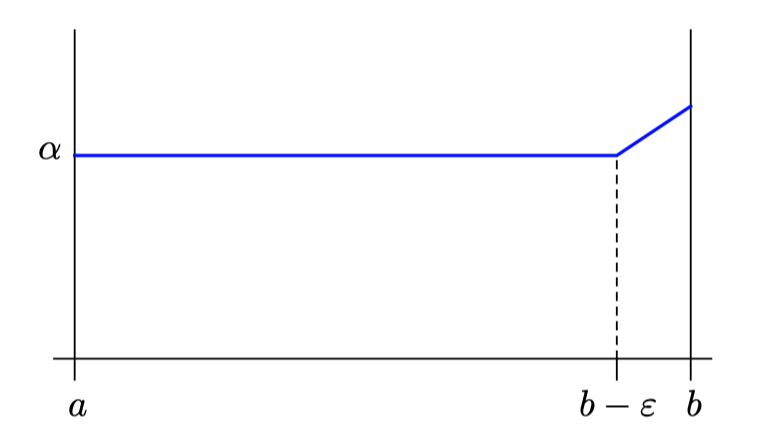
\includegraphics[width=0.5\textwidth]{Figs/a8.png}
    \caption{Perturbed Horizontal Line.}
    % \label{fig:Sawtooth}
\end{figure}

Its arc length
\begin{align*}
b-a+\varepsilon\left(\sqrt{1+\left(\frac{\alpha \beta+\gamma}{1-\varepsilon \beta}\right)^{2}}-1\right) \quad \longrightarrow \quad b-a
\end{align*}
as $\varepsilon \rightarrow 0 .$ One can even smooth off its corner, which has the effect of slightly decreasing its total arc length and thus does not affect the convergence as $\varepsilon \rightarrow 0$. Thus, while the 
Robin boundary value problem \tb{has no minimizing solution,} it does admit smooth functions that come arbitrarily close to the minimum possible value, which is $b-a$.
\end{exma} 
Similarly for  the brachistochrone problem \cref{exm:bra} with a free end, we can solve it using natural boundary condition and may also have conflict conditions.

\subsection{Null Lagrangians}
Despite the perhaps disappointing conclusion afforded by the inadmissibility of Robin conditions in \cref{exm:fdafadf}, it turns out it is possible to impose other types of boundary conditions on a variational principle, by suitably modifying the functional. With this aim, we first introduce an important notion of independent interest in the calculus of variations.
\begin{defa}\bfs{null Lagrangian}
A function $N(x, u, p)$ is called a \tb{null Lagrangian} if the gradient of its associated variational functional $K[u]=\int_{a}^{b} N\left(x, u, u^{\prime}\right) d x$ vanishes identically for all $u$: $\nabla K[u] \equiv 0$.
\end{defa} 
\begin{rema}
Null Lagrangians can be viewed as the calculus of variations equivalent of \tb{constant functions}, in that a function defined on a connected subset of $\mathbb{R}^{n}$ has zero gradient if and only if it is constant.
\end{rema}
\begin{exma}
Consider the variational problem
\begin{align*}
K[u]=\int_{0}^{\infty}\left[x^{2} u^{\prime}+2 x u\right] d x
\end{align*}
for the Lagrangian $N=x^{2} p+2 x u$. We compute its functional gradient using equation (3.12), and find
\begin{align*}
\nabla K[u]=\frac{\partial N}{\partial u}-\frac{d}{d x} \frac{\partial N}{\partial p}=2 x-\frac{d}{d x}\left(x^{2}\right) \equiv 0
\end{align*}
We conclude that $N$ is a null Lagrangian.
\end{exma}

Since the Euler-Lagrange equation of a null Lagrangian is simply $0=0$, every function satisfies it and thus, provided it also satisfies the imposed boundary conditions, is a critical function. We will shortly explain what this signifies. But first let us state an explicit characterization of all null Lagrangians.
\begin{thma}\label{thm:djcnadf}
A function $N(x, u, p)$ defined for all $(x, u, p) \in \mathbb{R}^{3}$ is \tb{a null Lagrangian} if and only if it is \tb{a total derivative}, so
\begin{align*}
N\left(x, u, u^{\prime}\right)=\frac{d}{d x} A(x, u)=\frac{\partial A}{\partial x}+u^{\prime} \frac{\partial A}{\partial u}
\end{align*}
for some function $A$ that depends only on $x, u$.
\end{thma} 
\begin{proof}
Referring back to the explicit form of the Euler-Lagrange equation \cref{eq:ndcdfadf}, the only term involving $u^{\prime \prime}$ is the last one, and so if the left hand side is to vanish for all possible functions $u(x)$, the coefficient of $u^{\prime \prime}$ must vanish, so 
$$\frac{\partial^{2} N}{\partial p^{2}}=0\text{ which implies }N(x, u, p)=f(x, u) p+g(x, u)$$
for some functions $f, g$. Substituting the latter expression back into \cref{eq:ndcdfadf} yields
\begin{align*}
u^{\prime} \frac{\partial f}{\partial u}+\frac{\partial g}{\partial u}-\frac{\partial f}{\partial x}-u^{\prime} \frac{\partial f}{\partial u}=\frac{\partial g}{\partial u}-\frac{\partial f}{\partial x}=0
\end{align*}
Since we are assuming $N$, and hence $f, g$ are defined for all $x, u$, a standard result of closed and exact form in \cite{rudin1976principles}[10.39 and 10.35], implies $f=\frac{\partial A}{\partial u}, g=\frac{\partial A}{\partial x}$, for some function $A(x, u)$.
\end{proof}
\begin{rema}
With \cref{thm:djcnadf} in hand, we can apply the Fundamental Theorem of Calculus to write the functional associated with a null Lagrangian in the following form:
\begin{align*}
J[u]=\int_{a}^{b} N\left(x, u, u^{\prime}\right) d x=\int_{a}^{b} \frac{d}{d x}[A(x, u)] d x=A(b, u(b))-A(a, u(a)) .
\end{align*}
In other words, \tb{the functional associated with a null Lagrangian depends only on the value of the function at the endpoints of the interval.} This explains why every function is in fact a minimizer (and maximizer) for null Lagrangian with fixed endpoints boundary condition.
\end{rema}
\subsection{General Boundary Conditions}
\subsubsection{Uncoupled Case}
So far we have treated fixed and free/natural boundary conditions, or combinations thereof. There exist uncoupled conflict conditions as shown in \cref{sec:dfadf}. However we can modify the original variational problem by adding in a suitable null Lagrangian, which \tb{does not alter the Euler-Lagrange equations but does change the associated natural boundary conditions.} In other words, if $N=D_{x} A$ is a null Lagrangian, then the modified objective functional
\begin{align*}
\begin{aligned}
\widetilde{J}[u] &=\int_{a}^{b}\left[L\left(x, u, u^{\prime}\right)+N\left(x, u, u^{\prime}\right)\right] d x=\int_{a}^{b}\left[L\left(x, u, u^{\prime}\right)+\frac{d}{d x}[A(x, u)]\right] d x \\
&=A(b, u(b))-A(a, u(a))+\int_{a}^{b} L\left(x, u, u^{\prime}\right) d x
\end{aligned}
\end{align*}
\tb{has the same Euler-Lagrange equations as $J[u]=\int_{a}^{b} L\left(x, u, u^{\prime}\right) d x$}.

\begin{enumerate}
    \item When subject to fixed boundary conditions, they have exactly the same critical functions, and hence the same minimizers, since their values differ only by the initial two boundary terms in the final expression, which depend only on the values of $u$ at the endpoints $a, b$. 
    \item On the other hand, as we will see, the two  problems have \tb{different natural boundary conditions}, and this flexibility allows us to convert any uncoupled boundary conditions into the variational framework.
\end{enumerate}

$\bullet$ \tb{New  Uncoupled Boundary Conditions:}

Uncoupled means we have separated conditions for the two ends. For simplicity, let's assume that  both boundary conditions explicitly involve the derivative of the function $u(x)$ at the endpoint: conditions for the derivative:
\begin{align}
u^{\prime}(a)=B_{1}(u(a)), \quad u^{\prime}(b)=B_{2}(u(b))\label{eq:dcfaf}
\end{align}
for some functions $B_{1}, B_{2}$ depending only on the value of $u$ at the endpoint in question.
\begin{rema}\bfs{two examples} In the following both cases,  $v(b)$ or $v(a)$ can take on \tb{any value}, according to the argument given above \cref{eq:dfadcyc}, they still satisfy the homogeneous natural boundary conditions.
\begin{enumerate}
    \item a free end with $B_{i}(u) \equiv 0$.
    \item another case of interest in a variety of physical situations are the aforementioned \tb{Robin boundary conditions}
\begin{align}
u^{\prime}(a)=\beta_{1} u(a)+\gamma_{1}, \quad u^{\prime}(b)=\beta_{2} u(b)+\gamma_{2}\label{eq:dvdfadfd}
\end{align}
in which $\beta_{1}, \beta_{2}, \gamma_{1}, \gamma_{2}$ are prescribed constants.
\end{enumerate}
\end{rema}

$\bullet$ \tb{What we want to do?}

Given a variational problem with Euler-Lagrange equation supplemented by the prescribed boundary conditions \cref{eq:dcfaf}, let us add in a suitable null Lagrangian  in order that \tb{the natural boundary conditions associated with the modified Lagrangian
\begin{align}
\widetilde{L}(x, u, p)=L(x, u, p)+N(x, u, p)=L(x, u, p)+p \frac{\partial A}{\partial u}(x, u)+\frac{\partial A}{\partial x}(x, u) \label{eq:dkncdfaf}
\end{align}
are ``equivalent'' to the desired boundary conditions \cref{eq:dcfaf}}.

At the right hand endpoint, in view of \cref{eq:dcfdfaf1}, this means
\begin{align*}
0=\frac{\partial \widetilde{L}}{\partial p}\left(b, u(b), u^{\prime}(b)\right)=\frac{\partial L}{\partial p}\left(b, u(b), u^{\prime}(b)\right)+\frac{\partial A}{\partial u}(b, u(b))
\end{align*}
is equivalent to the boundary equation $u^{\prime}(b)=B_{2}(u(b))$. For this to occur, we must require
\begin{align}
\frac{\partial A}{\partial u}(b, u(b))=-\frac{\partial L}{\partial p}\left(b, u(b), B_{2}(u(b))\right)\label{eq:dfadfod1}
\end{align}
Similarly, at the left hand endpoint, we require
\begin{align}
\frac{\partial A}{\partial u}(a, u(a))=-\frac{\partial L}{\partial p}\left(a, u(a), B_{1}(u(a))\right)\label{eq:dfadfod2}
\end{align}
These two conditions suffice to convert \cref{eq:dcfaf} as the natural boundary conditions for the variational problem associated with the modified Lagrangian \cref{eq:dkncdfaf}, thus justifying our claim that by adding in a suitable null Lagrangian $N=d A / d x$ we can \tb{arrange for any boundary conditions of the above form to be the natural boundary conditions associated with the variational problem.}
\begin{rema}
I think here we just get necessary conditions, while more assumptions may be needed to claim the equivalence.
\end{rema}

We can combine the conditions \cref{eq:dfadfod1} and \cref{eq:dfadfod2} into a simpler form as follows. Choose an "interpolating function" $B(x, u)$ such that
\begin{align*}
B(a, u(a))=B_{1}(u(a)), \quad B(b, u(b))=B_{2}(u(b)) .
\end{align*}
For example, we can use linear interpolation and set
\begin{align}
B(x, u)=\frac{x-a}{b-a} B_{2}(u)-\frac{x-b}{b-a} B_{1}(u)\label{eq:onmdfadfa}
\end{align}
In particular, if $B_{1}(u) \equiv B_{2}(u)$, so that we have the same boundary condition at both ends, we can set $B= B_1=B_2$.  \cref{eq:dfadfod1} and \cref{eq:dfadfod2}  are the implied by:
\begin{align}
    \frac{\partial A}{\partial u}(x, u)=-\frac{\partial L}{\partial p}(x, u, B(x, u)), \quad\text{ thus }\quad A(x, u)=-\int \frac{\partial L}{\partial p}(x, u, B(x, u)) d u\label{eq:domcdfa}
\end{align}

We have thus proved a general result about variational problems with specified boundary conditions:
\begin{thma}
Let $J[u]=\int_{a}^{b} L\left(x, u, u^{\prime}\right) d x$ be a variational problem whose minimizers are subject to the boundary conditions
\begin{align*}
u^{\prime}(a)=B(a, u(a)), \quad u^{\prime}(b)=B(b, u(b)),
\end{align*}
for some function $B(x, u)$. Let $A(x, u)$ be defined by \cref{eq:domcdfa}. Then the modified variational problem
\begin{align}
\widetilde{J}[u]=\int_{a}^{b}\left[L\left(x, u, u^{\prime}\right)+\frac{d}{d x} A(x, u)\right] d x=A(b, u(b))-A(a, u(a))+\int_{a}^{b} L\left(x, u, u^{\prime}\right) d x \label{eq:doncdfad}
\end{align}
has the same Euler-Lagrange equations and ``equivalent'' natural boundary conditions. 
\end{thma}
\begin{exma}
Let us consider the problem of minimizing arc length subject to the Robin boundary conditions \cref{eq:dvdfadfd} on the interval $[a, b]$. In accordance with \cref{eq:onmdfadfa}, set
$$B(x, u)=\beta(x) u+\gamma(x)\text{ where }\beta(x)=\frac{x-a}{b-a} \beta_{2}-\frac{x-b}{b-a} \beta_{1}, \gamma(x)=\frac{x-a}{b-a} \gamma_{2}-\frac{x-b}{b-a} \gamma_{1} .$$
Using the Lagrangian in \cref{sec:planargeo}, we compute
\begin{align*}
\frac{\partial L}{\partial p}=\frac{p}{\sqrt{1+p^{2}}}
\end{align*}
Substituting into \cref{eq:domcdfa}, the required function $A$ is obtained by integration:
\begin{align*}
A(x, u)=-\int \frac{\beta(x) u+\gamma(x)}{\sqrt{1+[\beta(x) u+\gamma(x)]^{2}}} d u=-\frac{\sqrt{1+[\beta(x) u+\gamma(x)]^{2}}}{\beta(x)}
\end{align*}
provided $\beta(x)\ne 0$. The modified variational problem \cref{eq:doncdfad} can thus be written as
 \begin{align}
\widetilde{J}[u] &=-\frac{\sqrt{1+\left[\beta_{2} u(b)+\gamma_{2}\right]^{2}}}{\beta_{2}}+\frac{\sqrt{1+\left[\beta_{1} u(a)+\gamma_{1}\right]^{2}}}{\beta_{1}}+\int_{a}^{b} \sqrt{1+u^{\prime}(x)^{2}} d x
\end{align}
Thus, while the basic arc length functional does not, in general, admit a minimizer that satisfies the Robin boundary conditions, the modified arc length (4.20), which has the same Euler-Lagrange equation, (usually) does. 

Let us solve the Robin boundary value problem for the Euler-Lagrange equation, which, as noted above, is merely $u^{\prime \prime}=0$, the solutions of which are straight lines $u=c x+d$. Substituting into the Robin boundary conditions \cref{eq:dvdfadfd} produces
\begin{align*}
c=\beta_{1}(c a+d)+\gamma_{1}=\beta_{2}(c b+d)+\gamma_{2}
\end{align*}
Accordingly, from the equations we have
\begin{enumerate}
    \item if
\begin{align*}
(b-a) \beta_{1} \beta_{2}+\beta_{2}-\beta_{1} \neq 0
\end{align*}
the problem admits a unique solution,
\item if the left hand side is zero, then there is either a one-parameter family of solutions that all give the same value to the modified variational problem (even though they have differing arc lengths), or there is no solution, depending on the values of  $\gamma_{1}, \gamma_{2}$.
\end{enumerate} 
\end{exma}
\subsubsection{Coupled Case}
Coupled boundary conditions relate the values of the minimizer and its derivatives at both endpoints? The simplest are the usual \tb{periodic boundary conditions}
\begin{align*}
u(a)=u(b), \quad u^{\prime}(a)=u^{\prime}(b)
\end{align*}
More generally we could try to impose a pair of coupled boundary conditions of the form
\begin{align*}
F_{i}\left(u(a), u^{\prime}(a), u(b), u^{\prime}(b)\right)=0, \quad i=1,2
\end{align*}
where each $F_{i}(u, p, v, q)$ depends on 4 arguments. The variation $v(x)$ will thus satisfy the linearization of each: \begin{align*} \frac{\partial F_{i}}{\partial u} v(a)+\frac{\partial F_{i}}{\partial p} v^{\prime}(a)+\frac{\partial F_{i}}{\partial v} v(b)+\frac{\partial F_{i}}{\partial q} v^{\prime}(b)=0 \end{align*}
We omit more discussion here.

\section{The Second Variation}\label{sec:secondvar}
The solutions to the Euler-Lagrange boundary value problem are the critical functions for the variational principle, meaning that they cause the functional gradient to vanish. 
\begin{enumerate}
    \item For finite-dimensional optimization problems, being a critical point is only a necessary condition for minimality. One must impose additional conditions, based on the \tb{second derivative} of the objective function at the critical point, in order to guarantee that it is a minimum and not a maximum or saddle point.
    \item Similarly, in the calculus of variations, the solutions to the Euler-Lagrange equation may also include (local) maxima, as well as other non-extremal critical functions. To distinguish between the possibilities, we need to formulate \tb{a second derivative }test for the objective functional. In the calculus of variations, the second derivative of a functional is known as its \tb{second variation}.
\end{enumerate} 
For a finite-dimensional objective function $F\left(u_{1}, \ldots, u_{n}\right)$, the second derivative test was based on the \tb{positive definiteness of its Hessian matrix.} 
The justification was based on the second order Taylor expansion of the objective function at the critical point. 

$\bullet$ \tb{Functional Taylor Expansion:}

In an analogous fashion, we expand an objective functional $J[u]$ near the critical function. Consider the scalar function
\begin{align*}
h(\varepsilon)=J[u+\varepsilon v]
\end{align*}
where the function $v(x)$ represents a variation. The second order Taylor expansion of $h(\varepsilon)$ takes the form
\begin{align*}
h(\varepsilon)=J[u+\varepsilon v]=J[u]+\varepsilon K[u ; v]+\frac{1}{2} \varepsilon^{2} Q[u ; v]+\cdots
\end{align*}
The first order terms are linear in the variation $v$, and, according to our earlier calculation, given by the inner product
\begin{align*}
h^{\prime}(0)=K[u ; v]=\langle\nabla J[u], v\rangle
\end{align*}
between the variation and the functional gradient. In particular, \tb{if $u$ is a critical function, then the first order terms vanish,}
\begin{align*}
K[u ; v]=\langle\nabla J[u], v\rangle=0
\end{align*}
for all allowable variations $v$, meaning those that satisfy the homogeneous boundary conditions. 

Therefore, the nature of the critical function $u$ - minimum, maximum, or neither - will, in most cases, be determined by the second derivative terms
\begin{align*}
h^{\prime \prime}(0)=Q[u ; v] .
\end{align*}
\tb{The crux of the second derivative test:}
\begin{enumerate}
    \item if $u$ is a minimizer, then $Q[u ; v] \geq 0$. 
    \item if $Q[u ; v]>0$ for all $v \not \equiv 0$, the second variation is positive definite, then the critical function $u$ will be a strict local minimizer. 
\end{enumerate}



Let us explicitly evaluate the second variational for \cref{eq:odnmfa}. Consider the scalar function
\begin{align*}
h(\varepsilon)=J[u+\varepsilon v]=\int_{a}^{b} L\left(x, u+\varepsilon v, u^{\prime}+\varepsilon v^{\prime}\right) d x
\end{align*}
whose first derivative $h^{\prime}(0)$ was already determined in \cref{eq:opdncdf}; here we require the second variation
\begin{align}
Q[u ; v]=h^{\prime \prime}(0)=\int_{a}^{b}\left[A v^{2}+2 B v v^{\prime}+C\left(v^{\prime}\right)^{2}\right] d x\label{eq:ddrdac}
\end{align}
where the coefficient functions
\begin{align}
A(x)=\frac{\partial^{2} L}{\partial u^{2}}\left(x, u, u^{\prime}\right), \quad B(x)=\frac{\partial^{2} L}{\partial u \partial p}\left(x, u, u^{\prime}\right), \quad C(x)=\frac{\partial^{2} L}{\partial p^{2}}\left(x, u, u^{\prime}\right)
\end{align}
are found by evaluating certain second order derivatives of the Lagrangian at the critical function $u(x)$.
\begin{rema}
In contrast to the first variation, integration by parts will not eliminate all of the derivatives on $v$ in the quadratic functional \cref{eq:ddrdac}, which causes significant complications in the ensuing analysis.
\end{rema}
The second derivative test for a minimizer relies on the \tb{positivity of the second variation}. So, in order to formulate conditions that the critical function be a minimizer for the functional, we need to establish criteria guaranteeing the positive definiteness of such a quadratic functional, meaning that $Q[u ; v]>0$ for all non-zero allowable variations $v(x) \not \equiv 0$. 

$\bullet$ \tb{A Strict Test:  pointwise positivity condition}

Clearly, if the integrand is \tb{positive definite at each point}, so
\begin{align}
    A(x) v^{2}+2 B(x) v v^{\prime}+C(x)\left(v^{\prime}\right)^{2}>0\text{  whenever }a<x<b, \text{ and }\quad v(x) \not \equiv 0\label{eq:donffvcz}
\end{align}
then $Q[u ; v]>0$ is also positive definite.
\begin{exma}
For the arc length minimization functional \cref{eq:odnfdaf}, the Lagrangian is $L(x, u, p)=\sqrt{1+p^{2}}$. To analyze the second variation, we first compute
\begin{align*}
\frac{\partial^{2} L}{\partial u^{2}}=0, \quad \frac{\partial^{2} L}{\partial u \partial p}=0, \quad \frac{\partial^{2} L}{\partial p^{2}}=\frac{1}{\left(1+p^{2}\right)^{3 / 2}}
\end{align*}
For the critical straight line function
\begin{align*}
u(x)=\frac{\beta-\alpha}{b-a}(x-a)+\alpha, \quad \text { with } \quad p=u^{\prime}(x)=\frac{\beta-\alpha}{b-a}
\end{align*}
we find
\begin{align*}
A(x)=\frac{\partial^{2} L}{\partial u^{2}}=0, \quad B(x)=\frac{\partial^{2} L}{\partial u \partial p}=0, \quad C(x)=\frac{\partial^{2} L}{\partial p^{2}}=\frac{(b-a)^{3}}{\left[(b-a)^{2}+(\beta-\alpha)^{2}\right]^{3 / 2}} \equiv c .
\end{align*}
Therefore, the second variation functional \cref{eq:ddrdac} is
\begin{align*}
Q[u ; v]=\int_{a}^{b} c\left(v^{\prime}\right)^{2} d x
\end{align*}
where $c>0$ is a positive constant. Thus, $Q[u ; v]=0$ vanishes if and only if $v(x)$ is a constant function. But the variation $v(x)$ is required to satisfy the homogeneous boundary conditions $v(a)=v(b)=0$, and hence $Q[u ; v]>0$ for all allowable nonzero variations. Therefore, we conclude that the straight line is, indeed, a (local) minimizer for the arc length functional.
\end{exma}


However, as the following example demonstrates, the pointwise positivity condition \cref{eq:donffvcz} is overly restrictive.
\begin{exma}
Consider the quadratic functional
\begin{align}
Q[v]=\int_{0}^{1}\left[\left(v^{\prime}\right)^{2}-v^{2}\right] d x \label{eq:dkcnafdas}
\end{align}
We claim that $Q[v]>0$ for all nonzero $v \not \equiv 0$ subject to \tb{homogeneous Dirichlet boundary conditions}
$$v(0)=0=v(1).$$ The boundary conditions play an essential role, since choosing $v(x) \equiv c \neq 0$ to be any constant function will produce a negative value for the functional: $Q[v]=-c^{2}$.
To prove the claim, consider the quadratic functional
\begin{align*}
\widetilde{Q}[v]=\int_{0}^{1}\left(v^{\prime}+v \tan x\right)^{2} d x \geq 0
\end{align*}
which is clearly non-negative, since the integrand is everywhere $\geq 0$. Moreover, by continuity, the integral vanishes if and only if $v$ satisfies the first order linear ordinary differential equation
\begin{align*}
v^{\prime}+v \tan x=0, \quad \text { for all } \quad 0 \leq x \leq 1
\end{align*}
The only solution that also satisfies boundary condition $v(0)=0$ is the trivial one $v \equiv 0$. We conclude that $\widetilde{Q}[v]=0$ if and only if $v \equiv 0$, and hence $\widetilde{Q}[v]$ is a positive definite quadratic functional on the space of allowable variations.
Let us expand the latter functional,
\begin{align*}
\begin{aligned}
\widetilde{Q}[v] &=\int_{0}^{1}\left[\left(v^{\prime}\right)^{2}+2 v v^{\prime} \tan x+v^{2} \tan ^{2} x\right] d x \\
&=\int_{0}^{1}\left[\left(v^{\prime}\right)^{2}-v^{2}(\tan x)^{\prime}+v^{2} \tan ^{2} x\right] d x=\int_{0}^{1}\left[\left(v^{\prime}\right)^{2}-v^{2}\right] d x=Q[v]
\end{aligned}
\end{align*}
In the second equality, we integrated the middle term by parts, using $\left(v^{2}\right)^{\prime}=2 v v^{\prime}$, and noting that the boundary terms vanish owing to our imposed boundary conditions. Since $\widetilde{Q}[v]$ is positive definite, so is $Q[v]$, justifying the previous claim.
\end{exma} 
\begin{rema}
To appreciate how delicate this result is, consider the almost identical quadratic functional
\begin{align}
\widehat{Q}[v]=\int_{0}^{4}\left[\left(v^{\prime}\right)^{2}-v^{2}\right] d x\label{eq:dincdfafd}
\end{align}
the only difference being the upper limit of the integral. A quick computation shows that the function $v(x)=x(4-x)$ satisfies the boundary conditions $v(0)=0=v(4)$, but
\begin{align*}
\widehat{Q}[v]=\int_{0}^{4}\left[(4-2 x)^{2}-x^{2}(4-x)^{2}\right] d x=-\frac{64}{5}<0
\end{align*}
Therefore, $\widehat{Q}[v]$ is not positive definite. Our preceding analysis does not apply because the function $\tan x$ becomes singular at $x=\frac{1}{2} \pi$, and so the auxiliary integral $\int_{0}^{4}\left(v^{\prime}+v \tan x\right)^{2} d x$ does not converge.
\end{rema}


\subsection{Fundamental Theorem}
The complete analysis of positive definiteness of quadratic functionals is quite subtle. Indeed, the strange appearance of $\tan x$ in the preceding example turns out to be an important clue! In the interests of brevity, let us just state without proof a fundamental theorem:
\begin{thma}\label{thm:dccda}
Let $A(x), B(x), C(x) \in \mathrm{C}^{0}[a, b]$ be continuous functions. The quadratic functional
\begin{align*}
Q[v]=\int_{a}^{b}\left[A v^{2}+2 B v v^{\prime}+C\left(v^{\prime}\right)^{2}\right] d x
\end{align*}
is positive definite, so $Q[v]>0$ for all $v \not \equiv 0$ satisfying the homogeneous Dirichlet boundary
conditions $v(a)=v(b)=0$, provided 
\begin{enumerate}[(a).]
    \item $C(x)>0$ for all $a \leq x \leq b$, and
    \item For any $a<c \leq b$, the only solution to its linear Euler-Lagrange boundary value problem
\begin{align}
-\left(C v^{\prime}\right)^{\prime}+\left(A-B^{\prime}\right) v=0, \quad v(a)=0=v(c) \label{eq:dkincda}
\end{align}
is the trivial function $v(x) \equiv 0$.
\end{enumerate}
\end{thma}
\begin{rema}\bfs{conjugate point}
A value $c$ for which \cref{eq:dkincda} has a nontrivial solution is known as a conjugate point to $a$. Thus, condition (b) can be restated that the variational problem has no conjugate points in the interval $(a, b]$.
\end{rema}
\begin{exma}
The quadratic functional
\begin{align}
Q[v]=\int_{0}^{b}\left[\left(v^{\prime}\right)^{2}-v^{2}\right] d x\label{eq:dcmmxd}
\end{align}
has Euler-Lagrange equation
\begin{align*}
-v^{\prime \prime}-v=0
\end{align*}
The solutions $v(x)=k \sin x$ satisfy the boundary condition $v(0)=0$. The first conjugate point occurs at $c=\pi$ where $v(\pi)=0$. Therefore, \cref{thm:dccda} implies that the quadratic functional \cref{eq:dcmmxd} is positive definite provided the upper integration limit $b<\pi$. This explains why the original quadratic functional \cref{eq:dkcnafdas}is positive definite, since there are no conjugate points on the interval $[0,1]$, while the modified version \cref{eq:dincdfafd} is not, because the first conjugate point $\pi$ lies on the interval $(0,4]$.
\end{exma}

$\bullet$ \tb{Special Case for \cref{eq:odnmfa}:}

In the case when the quadratic functional arises as the second variation of a functional \cref{eq:odnmfa}, the coefficient functions $A, B, C$ are given in terms of the Lagrangian $L(x, u, p)$ by formulae \cref{eq:ddrdac}.  \cref{thm:dccda} requires
\begin{enumerate}
    \item First condition:\begin{align}
\frac{\partial^{2} L}{\partial p^{2}}\left(x, u, u^{\prime}\right)>0 \label{eq:dkcdfa}
\end{align}
for the candidate minimizer $u(x)$ that solves the Euler-Lagrange equation. This is known as the \tb{Legendre condition}.
\item  The second, conjugate point condition requires that the so-called \tb{linearized variational equation}
\begin{align}
-\frac{d}{d x}\left[\frac{\partial^{2} L}{\partial p^{2}}\left(x, u, u^{\prime}\right) \frac{d v}{d x}\right]+\left[\frac{\partial^{2} L}{\partial u^{2}}\left(x, u, u^{\prime}\right)-\frac{d}{d x} \frac{\partial^{2} L}{\partial u \partial p}\left(x, u, u^{\prime}\right)\right] v=0 \label{eq:dacdffd}
\end{align}
where $u(x)$ is the candidate minimizer, has no nontrivial solutions $v(x) \not \equiv 0$ that satisfy $v(a)=0$ and $v(c)=0$ for $a<c \leq b$. 
\end{enumerate}
In this way, we have arrived at a rigorous form of the second derivative test for the simplest functional in the calculus of variations.

\begin{thma}
If the function $u(x)$ satisfies the Euler-Lagrange equation \cref{eq:ndcdfadf}, and, in addition, the Legendre condition \cref{eq:dkcdfa} holds and there are no conjugate points for \cref{eq:dacdffd} on the interval, then $u(x)$ is a \tb{strict local minimum} for the functional.
\end{thma} 
\section{Multi-dimensional Variational Problems}
The calculus of variations encompasses a very broad range of mathematical applications. The methods of variational analysis can be applied to an enormous variety of physical systems, whose \tb{equilibrium configurations inevitably minimize a suitable functional, which, typically, represents the potential energy of the system.} Minimizing configurations appear as critical functions at which the functional gradient vanishes. Following similar computational procedures as in the one-dimensional calculus of variations, we find that the \tb{critical functions are characterized as solutions to a system of partial differential equations, known as the Euler-Lagrange equations associated with the variational principle.} Each solution to the boundary value problem specified by the Euler-Lagrange equations subject to appropriate boundary conditions is, thus, a candidate minimizer for the variational problem. 
\begin{rema}
In many applications, the Euler-Lagrange boundary value problem suffices to single out the physically relevant solutions, and one need not press on to the considerably more difficult second variation.
\end{rema}
$\bullet$ \tb{two variables case}

We consider a first order variational problem involving a single scalar function of two variables. Once this is fully understood, generalizations and extensions to higher dimensions and higher order Lagrangians are readily apparent.

$\bullet$ \tb{Objective Functional:}
\begin{align*}
J[u]=\iint_{\Omega} L\left(x, y, u, u_{x}, u_{y}\right) d x d y
\end{align*}
having the form of a double integral over a prescribed domain $\Omega \subset \mathbb{R}^{2}$. The \tb{Lagrangian} $L(x, y, u, p, q)$ is assumed to be a sufficiently smooth function of its five arguments. 

$\bullet$ \tb{Boundary Condition:}

Our goal is to find the function(s) $u=f(x, y)$ that minimize the value of $J[u]$ when subject to a set of prescribed boundary conditions on $\partial \Omega$, the most important being our usual Dirichlet, Neumann, or mixed boundary conditions. 

For simplicity, we concentrate on the \tb{Dirichlet boundary value problem}, and require that the minimizer satisfy
\begin{align*}
u(x, y)=g(x, y) \quad \text { for } \quad(x, y) \in \partial \Omega .
\end{align*}

\subsection{The First Variation and the Euler-Lagrange Equations}
Similar to the one-dim case, consider the scalar function
\begin{align}
h(\varepsilon) \equiv J[u+\varepsilon v]=\iint_{\Omega} L\left(x, y, u+\varepsilon v, u_{x}+\varepsilon v_{x}, u_{y}+\varepsilon v_{y}\right) d x d y\label{eq:dojancfadf}
\end{align}
depending on $\varepsilon \in \mathbb{R}$. The \tb{variation} $v(x, y)$ is assumed to satisfy \tb{homogeneous Dirichlet boundary conditions} \begin{align*} v(x, y)=0 \quad \text { for } \quad(x, y) \in \partial \Omega \end{align*} conditions, if $u$ is a minimizer, then the scalar function $h(\varepsilon)$ will have a minimum at $\varepsilon=0$, and hence
\begin{align*}
h^{\prime}(0)=0 \text {. }
\end{align*}
When computing $h^{\prime}(\varepsilon)$, we assume that the functions involved are sufficiently as to allow us to bring the derivative inside the integral, and then apply the chai $\varepsilon=0$, the result is
\begin{align} h^{\prime}(0)=\left.\frac{d}{d \varepsilon} J[u+\varepsilon v]\right|_{\varepsilon=0}=\iint_{\Omega}\left(v \frac{\partial L}{\partial u}+v_{x} \frac{\partial L}{\partial p}+v_{y} \frac{\partial L}{\partial q}\right) d x d y \label{eq:doncadf}
\end{align}
where the derivatives of $L$ are all evaluated at $x, y, u, u_{x}, u_{y} .$ To identify the functional gradient, we need to rewrite this integral in the form of an inner product: \begin{align*} h^{\prime}(0)=\langle\nabla J[u], v\rangle=\iint_{\Omega} h(x, y) v(x, y) d x d y, \quad \text { where } h=\nabla J[u] \end{align*}
To convert \cref{eq:doncadf} into this form, we need to remove the offending derivatives from $v$. In two dimensions, the requisite integration by parts formula is based on \tb{Green's Theorem}:
\begin{thma}\bfs{Green's Theorem}\label{thm:idnacc}
\begin{align*}
\iint_{\Omega}\left(\frac{\partial v}{\partial x} w_{1}+\frac{\partial v}{\partial y} w_{2}\right) d x d y=\oint_{\partial \Omega} v\left(-w_{2} d x+w_{1} d y\right)-\iint_{\Omega} v\left(\frac{\partial w_{1}}{\partial x}+\frac{\partial w_{2}}{\partial y}\right) d x d y
\end{align*}
in which $w_{1}, w_{2}$ are arbitrary smooth functions. 
\end{thma}
Apply the Green's Theorem, we get that with $w_{1}=\frac{\partial L}{\partial p}$, $w_{2}=\frac{\partial L}{\partial q}$, we find $\iint_{\Omega}\left(v_{x} \frac{\partial L}{\partial p}+v_{y} \frac{\partial L}{\partial q}\right) d x d y=-\iint_{\Omega} v\left[\frac{\partial}{\partial x}\left(\frac{\partial L}{\partial p}\right)+\frac{\partial}{\partial y}\left(\frac{\partial L}{\partial q}\right)\right] d x d y$
where the boundary integral vanishes owing to the boundary conditions \cref{eq:dojancfadf} that we impose on the allowed variations. Substituting this result back into \cref{eq:doncadf}, we conclude that
\begin{align*}
h^{\prime}(0)=\iint_{\Omega} v\left[\frac{\partial L}{\partial u}-\frac{\partial}{\partial x}\left(\frac{\partial L}{\partial p}\right)-\frac{\partial}{\partial y}\left(\frac{\partial L}{\partial q}\right)\right] d x d y=\langle\nabla J[u], v\rangle
\end{align*}
where
\begin{align*}
\nabla J[u]=\frac{\partial L}{\partial u}-\frac{\partial}{\partial x}\left(\frac{\partial L}{\partial p}\right)-\frac{\partial}{\partial y}\left(\frac{\partial L}{\partial q}\right)
\end{align*}
is the desired first variation or functional gradient. 

$\bullet$ \tb{Euler-Lagrange equation:}

Since the gradient vanishes at a critical function, we conclude that the minimizer $u(x, y)$ must satisfy the \tb{Euler-Lagrange equation} 
\begin{align}
    \frac{\partial L}{\partial u}\left(x, y, u, u_{x}, u_{y}\right)-\frac{\partial}{\partial x}\left(\frac{\partial L}{\partial p}\left(x, y, u, u_{x}, u_{y}\right)\right)-\frac{\partial}{\partial y}\left(\frac{\partial L}{\partial q}\left(x, y, u, u_{x}, u_{y}\right)\right)=0 .
\end{align}
Once we explicitly evaluate the derivatives, the net result is a second order partial differential equation
$$L_{u}-L_{x p}-L_{y q}-u_{x} L_{u p}-u_{y} L_{u q}-u_{x x} L_{p p}-2 u_{x y} L_{p q}-u_{y y} L_{q q}=0$$ where we use subscripts to indicate derivatives of both $u$ and $L$, the latter being evaluated at $x, y, u, u_{x}, u_{y} .$ 
\begin{exma}
As a first elementary example, consider the Dirichlet minimization \begin{align*} J[u]=\iint_{\Omega} \frac{1}{2}\left(u_{x}^{2}+u_{y}^{2}\right) d x d y \end{align*} at $x, y, u, u_{x}, u_{y}$.
As a first elementary example, consider the Dirichlet minimization problem
In this case, the associated Lagrangian is \begin{align*} L=\frac{1}{2}\left(p^{2}+q^{2}\right), \quad \text { with } \quad \frac{\partial L}{\partial u}=0, \quad \frac{\partial L}{\partial p}=p=u_{x}, \quad \frac{\partial L}{\partial q}=q=u_{y} \end{align*}
\begin{align*}
-\frac{\partial}{\partial x}\left(u_{x}\right)-\frac{\partial}{\partial y}\left(u_{y}\right)=-u_{x x}-u_{y y}=-\Delta u=0
\end{align*}
which is the two-dimensional Laplace equation. Subject to the selected boundary conditions, the solutions, i.e., the harmonic functions, are critical functions for the Dirichlet variational principle.
\end{exma} 
\begin{rema}
Again,  so far we only have candidates for minimizing the Dirichlet integral; they could just as easily be maximizing functions or saddle points.
\end{rema}

\begin{exma}
 Let us derive the Euler-Lagrange equation for the minimal surface problem. From \cref{eq:Ldfds}, the surface area integral
$J[u]=\iint_{\Omega} \sqrt{1+u_{x}^{2}+u_{y}^{2}} d x d y \quad$ has Lagrangian $\quad L=\sqrt{1+p^{2}+q^{2}}$
Note that
\begin{align*}
\frac{\partial L}{\partial u}=0, \quad \frac{\partial L}{\partial p}=\frac{p}{\sqrt{1+p^{2}+q^{2}}}, \quad \frac{\partial L}{\partial q}=\frac{q}{\sqrt{1+p^{2}+q^{2}}}
\end{align*}
Therefore, replacing $p \rightarrow u_{x}$ and $q \rightarrow u_{y}$ and then evaluating the derivatives, the Euler Lagrange equation  becomes
\begin{align*}
-\frac{\partial}{\partial x} \frac{u_{x}}{\sqrt{1+u_{x}^{2}+u_{y}^{2}}}-\frac{\partial}{\partial y} \frac{u_{y}}{\sqrt{1+u_{x}^{2}+u_{y}^{2}}}=\frac{-\left(1+u_{y}^{2}\right) u_{x x}+2 u_{x} u_{y} u_{x y}-\left(1+u_{x}^{2}\right) u_{y y}}{\left(1+u_{x}^{2}+u_{y}^{2}\right)^{3 / 2}}=0
\end{align*}
Thus, a surface described by the graph of a function $u=f(x, y)$ is a critical function, and hence a candidate for minimizing surface area, provided it satisfies the minimal surface equation
\begin{align*}
\left(1+u_{y}^{2}\right) u_{x x}-2 u_{x} u_{y} u_{x y}+\left(1+u_{x}^{2}\right) u_{y y}=0
\end{align*}
We are confronted with a complicated, nonlinear, second order partial differential equation, which has been the focus of some of the most sophisticated and deep analysis over the past two centuries, with significant progress on understanding its solution only within the past 70 years. We refer the interested reader to the advanced texts or further developments in this fascinating area of mathematical analysis.
\end{exma}
\begin{exma}
  The deformations of an elastic body $\Omega \subset \mathbb{R}^{n}$ are described by the displacement field, $\mathbf{u :} \Omega \rightarrow \mathbb{R}^{n} .$ Each material point $\mathbf{x} \in \Omega$ in the undeformed body will move to a new position $\mathbf{y}=\mathbf{x}+\mathbf{u}(\mathbf{x})$ in the deformed body
\begin{align*}
\widetilde{\Omega}=\{\mathbf{y}=\mathbf{x}+\mathbf{u}(\mathbf{x}) \mid \mathbf{x} \in \Omega\}
\end{align*}
The one-dimensional case governs bars, beams and rods, two-dimensional bodies include thin plates and shells, while $n=3$ for fully three-dimensional solid bodies. 

For small deformations, we can use a linear theory to approximate the much more complicated equations of nonlinear elasticity. The simplest case is that of a homogeneous and isotropic planar body $\Omega \subset \mathbb{R}^{2} .$ The equilibrium configurations are described by the deformation function $\mathbf{u}(\mathbf{x})=(u(x, y), v(x, y))$. A detailed physical analysis of the constitutive assumptions leads to a minimization principle based on the following functional:
\begin{align}
\begin{aligned}
J[u, v] &=\iint_{\Omega}\left[\frac{1}{2} \mu\|\nabla \mathbf{u}\|^{2}+\frac{1}{2}(\lambda+\mu)(\nabla \cdot \mathbf{u})^{2}\right] d x d y \\
&=\iint_{\Omega}\left[\left(\frac{1}{2} \lambda+\mu\right)\left(u_{x}^{2}+v_{y}^{2}\right)+\frac{1}{2} \mu\left(u_{y}^{2}+v_{x}^{2}\right)+(\lambda+\mu) u_{x} v_{y}\right] d x d y \label{eq:doafdaf}
\end{aligned}
\end{align}
The parameters $\lambda, \mu$ are known as the Lamé moduli of the material, and govern its intrinsic elastic properties. They are measured by performing suitable experiments on a sample of the material. Physically, \cref{eq:doafdaf} represents the stored (or potential) energy in the body under the prescribed displacement. \tb{Nature, as always, seeks the displacement that will minimize the total energy.}

To compute the \tb{Euler-Lagrange equations}, we consider the functional variation
\begin{align*}
h(\varepsilon)=J[u+\varepsilon f, v+\varepsilon g]
\end{align*}
in which the individual variations $f, g$ are arbitrary functions subject only to the given homogeneous boundary conditions. If $u, v$ minimize $J$, then $h(\varepsilon)$ has a minimum at $\varepsilon=0$, and so we are led to compute
\begin{align*}
h^{\prime}(0)=\langle\nabla J, \mathbf{f}\rangle=\iint_{\Omega}\left(f \nabla_{u} J+g \nabla_{v} J\right) d x d y
\end{align*}
which we write as an inner product (using the standard $\mathrm{L}^{2}$ inner product between vector fields ) between the variation $\mathbf{f}=(f,g)$ and the functional gradient $\nabla J=\left(\nabla_{u} J, \nabla_{v} J\right) .$ For the particular functional \cref{eq:doafdaf}, we find
\begin{align*}
h^{\prime}(0)=\iint_{\Omega}\left[(\lambda+2 \mu)\left(u_{x} f_{x}+v_{y} g_{y}\right)+\mu\left(u_{y} f_{y}+v_{x} g_{x}\right)+(\lambda+\mu)\left(u_{x} g_{y}+v_{y} f_{x}\right)\right] d x d y .
\end{align*}
We use the integration by parts formula \cref{thm:idnacc} to remove the derivatives from the variations $f, g .$ Discarding the boundary integrals, which are used to prescribe the allowable boundary conditions, we find
\begin{align*}
h^{\prime}(0)=-\iint_{\Omega}\left(\begin{array}{r}
{\left[(\lambda+2 \mu) u_{x x}+\mu u_{y y}+(\lambda+\mu) v_{x y}\right] f} \\
+\left[(\lambda+\mu) u_{x y}+\mu v_{x x}+(\lambda+2 \mu) v_{y y}\right] g
\end{array}\right) d x d y
\end{align*}
The two terms in brackets give the two components of the functional gradient. Setting them equal to zero, we derive the second order linear system of Euler-Lagrange equations
\begin{align*}
\begin{aligned}
&(\lambda+2 \mu) u_{x x}+\mu u_{y y}+(\lambda+\mu) v_{x y}=0 \\
&(\lambda+\mu) u_{x y}+\mu v_{x x}+(\lambda+2 \mu) v_{y y}=0
\end{aligned}
\end{align*}
known as Navier's equations, which can be compactly written as
\begin{align*}
\mu \Delta \mathbf{u}+(\mu+\lambda) \nabla(\nabla \cdot \mathbf{u})=\mathbf{0}
\end{align*}
for the displacement vector $\mathbf{u}=(u, v)$. The solutions to are the critical displacements that, under appropriate boundary conditions, minimize the potential energy functional.
Since we are dealing with a quadratic functional, a more detailed algebraic analysis will demonstrate that the solutions to Navier's equations are the minimizers for the variational principle \cref{eq:doafdaf}. Although only valid in a limited range of physical and kinematical conditions, the solutions to the planar Navier's equations and its three-dimensional counterpart are successfully used to model a wide class of elastic materials.
\end{exma}

In general, the solutions to the Euler-Lagrange boundary value problem are critical functions for the variational problem, and hence include all (smooth) local and global minimizers. Determination of which solutions are genuine minima requires a further analysis of the positivity properties of the second variation, which is beyond the scope of our introductory treatment. Indeed, a complete analysis of the positive definiteness of the second variation of multi-dimensional variational problems is quite complicated, and still awaits a completely satisfactory resolution!
\bibliographystyle{IEEEtran}
\bibliography{IEEEabrv,StringDefinitions,adv_dnn}
\end{document}